%%%%%%%%%%%%%%%%%%%%%%%%%%%%%%%%%%%%%%%%%
% Short Sectioned Assignment LaTeX Template Version 1.0 (5/5/12)
% This template has been downloaded from: http://www.LaTeXTemplates.com
% Original author:  Frits Wenneker (http://www.howtotex.com)
% License: CC BY-NC-SA 3.0 (http://creativecommons.org/licenses/by-nc-sa/3.0/)
%%%%%%%%%%%%%%%%%%%%%%%%%%%%%%%%%%%%%%%%%

% \documentclass[paper=a4, fontsize=11pt]{scrartcl} % A4 paper and 11pt font size
\documentclass[11pt, a4paper]{book}
\usepackage[T1]{fontenc} % Use 8-bit encoding that has 256 glyphs
\usepackage[utf8]{inputenc}
\usepackage{fourier} % Use the Adobe Utopia font for the document - comment this line to return to the LaTeX default
\usepackage{listings} % para insertar código con formato similar al editor
\usepackage[spanish, es-tabla]{babel} % Selecciona el español para palabras introducidas automáticamente, p.ej. "septiembre" en la fecha y especifica que se use la palabra Tabla en vez de Cuadro
\usepackage{url} % ,href} %para incluir URLs e hipervínculos dentro del texto (aunque hay que instalar href)
\usepackage{graphics,graphicx, float} %para incluir imágenes y colocarlas
\usepackage[gen]{eurosym} %para incluir el símbolo del euro
\usepackage{cite} %para incluir citas del archivo <nombre>.bib
\usepackage{enumerate}
\usepackage{hyperref}
\usepackage{graphicx}
\usepackage{tabularx}
\usepackage{booktabs}
\usepackage{pdflscape}

\usepackage[table,xcdraw]{xcolor}
\hypersetup{
	colorlinks=true,	% false: boxed links; true: colored links
	linkcolor=black,	% color of internal links
	urlcolor=cyan		% color of external links
}
\renewcommand{\familydefault}{\sfdefault}
\usepackage{fancyhdr} % Custom headers and footers
\pagestyle{fancyplain} % Makes all pages in the document conform to the custom headers and footers
\fancyhead[L]{} % Empty left header
\fancyhead[C]{} % Empty center header
\fancyhead[R]{Elena Ortega Contreras} % My name
\fancyfoot[L]{} % Empty left footer
\fancyfoot[C]{} % Empty center footer
\fancyfoot[R]{\thepage} % Page numbering for right footer
%\renewcommand{\headrulewidth}{0pt} % Remove header underlines
\renewcommand{\footrulewidth}{0pt} % Remove footer underlines
\setlength{\headheight}{13.6pt} % Customize the height of the header

\usepackage{titlesec, blindtext, color}
\definecolor{gray75}{gray}{0.75}
\newcommand{\hsp}{\hspace{20pt}}
\titleformat{\chapter}[hang]{\Huge\bfseries}{\thechapter\hsp\textcolor{gray75}{|}\hsp}{0pt}{\Huge\bfseries}
\setcounter{secnumdepth}{4}
\usepackage[Lenny]{fncychap}



\begin{document}

	% Plantilla portada UGR
	\begin{titlepage}
    \newlength{\centeroffset}
    \setlength{\centeroffset}{-0.5\oddsidemargin}
    \addtolength{\centeroffset}{0.5\evensidemargin}
    \thispagestyle{empty}
    
    \noindent\hspace*{\centeroffset}
    \begin{minipage}{\textwidth}
    
    \centering
    
\includegraphics[width=0.9\textwidth]{logos/logo_ugr.jpg}\\[1.4cm]
    
    \textsc{ \Large TRABAJO FIN DE GRADO\\[0.2cm]}
    \textsc{ GRADO EN INGENIERIA INFORMATICA}\\[1cm]
    
    {\Huge\bfseries SIGMA \\}
    \noindent\rule[-1ex]{\textwidth}{3pt}\\[3.5ex]
    {\large\bfseries Sistema Inteligente de Gestión Monetaria Automatizada }
    \end{minipage}
    
    \vspace{2.5cm}
    \noindent\hspace*{\centeroffset}
    \begin{minipage}{\textwidth}
    \centering
    
    \textbf{Autor}\\ {Elena Ortega Contreras}\\[2.5ex]
    \textbf{Director}\\ {José Manuel Soto García}\\[2cm]
    
\includegraphics[width=0.3\textwidth]{logos/etsiit_logo.png}\\[0.1cm]
    \textsc{Escuela Técnica Superior de Ingenierías Informática y de Telecomunicación}\\
    \textsc{---}\\
    Granada, Junio de 2024
    \end{minipage}
    \end{titlepage}

	% Plantilla prefacio UGR
	\thispagestyle{empty}

\begin{center}
{\large\bfseries Título \\ Subtítulo }\\
\end{center}
\begin{center}
Nombre Del Estudiante\\
\end{center}

%\vspace{0.7cm}

\vspace{0.5cm}
\noindent\textbf{Palabras clave}: \textit{software libre}
\vspace{0.7cm}

\noindent\textbf{Resumen}\\
	

\cleardoublepage

\begin{center}
	{\large\bfseries Same, but in English}\\
\end{center}
\begin{center}
	Student's name\\
\end{center}
\vspace{0.5cm}
\noindent\textbf{Keywords}: \textit{open source}, \textit{floss}
\vspace{0.7cm}

\noindent\textbf{Abstract}\\


\cleardoublepage

\thispagestyle{empty}

\noindent\rule[-1ex]{\textwidth}{2pt}\\[4.5ex]

D. \textbf{Tutora/e(s)}, Profesor(a) del ...

\vspace{0.5cm}

\textbf{Informo:}

\vspace{0.5cm}

Que el presente trabajo, titulado \textit{\textbf{Chief}},
ha sido realizado bajo mi supervisión por \textbf{Estudiante}, y autorizo la defensa de dicho trabajo ante el tribunal
que corresponda.

\vspace{0.5cm}

Y para que conste, expiden y firman el presente informe en Granada a Junio de 2018.

\vspace{1cm}

\textbf{El/la director(a)/es: }

\vspace{5cm}

\noindent \textbf{(nombre completo tutor/a/es)}

\chapter*{Agradecimientos}

Poner aquí agradecimientos...



	% Índice de contenidos
	\newpage
	\tableofcontents

	% Índice de imágenes y tablas
	\newpage
	\listoffigures

	% Si hay suficientes se incluirá dicho índice
	\listoftables 
	\newpage

	% Introducción 
	\chapter{Introducción}
En esta sección se detalla la importancia de la gestión económica personal y cómo el avance de la digitalización ha transformado la manera en que interactuamos con nuestras finanzas. Se presenta un recorrido por la evolución de los servicios financieros digitales en España, desde los primeros cajeros automáticos hasta las modernas formas de pago como \textit{Bizum} y \textit{NFC}. Asimismo, se analizan los retos actuales que enfrentan los usuarios al gestionar sus finanzas personales, dadas las múltiples fuentes de ingresos y métodos de pago disponibles. Se explora cómo las soluciones \textit{Fintech} han surgido para abordar estos desafíos.

\section{Contexto. Descripción del problema} 
Según su definición en la \href{https://dle.rae.es/economía}{RAE} la economía es la 
\textit{Administración eficaz y razonable de los bienes}, dicho esto y teniendo en 
cuenta que nos concierne a todos, es crucial tener control sobre ella. 
De manera individual, las decisiones financieras influyen en la calidad de vida de las personas,
un uso adecuado es esencial para evitar problemas como el endeudamiento, la 
falta de ahorro o la incapacidad de cumplir metas económicas.

La transición hacia lo digital está cambiando nuestra forma de interactuar con 
la información, nos permite realizar tareas de forma remota, rápida y eficiente. 
En los últimos años, en España la banca ha evolucionado rápidamente hacia lo digital, comenzando en los años 70 con la introducción de cajeros automáticos. En los 80, las tecnologías de la información mejoraron la eficiencia de los mercados financieros, y en los 90, surgieron los primeros servicios bancarios a distancia, como la banca telefónica. En 1995, se lanzó el primer software que permitía ver finanzas online, y en 1999 los bancos españoles comenzaron a ofrecer sus primeros servicios de consulta online. A partir del año 2006 la llegada de los smartphones y la evolución de Internet aceleraron la transformación \cite{hebrero2022fintech}.

Actualmente, esta digitalización ha brindado la posibilidad de utilizar diversas formas de de pago como transferencias bancarias, el uso de tarjetas de crédito, sistemas de pago instantáneo como \href{https://bizum.es/}{Bizum}, pago con dispositivos como smartphones y relojes inteligentes mediante NFC \footnote{NFC (Near Field Communication) es una tecnología que permite una comunicación de corto alcance entre dispositivos inhalámbricos para intercambiar pequeñas cantidades de datos} y un largo etcétera. Por supuesto, no podemos olvidar el uso de dinero en efectivo, que sigue siendo una forma de pago común. 

En una época en la que los precios son muy elevados, pero a la vez el consumo parece estar desvocado, es importante administrar el dinero de manera responsable. Esto implica planificación y control sobre cómo y dónde lo gastamos.
Sin embargo, no es fácil hacer el seguimiento de las finanzas personales ya que se 
juntan diversos factores a tener en cuenta: podemos tener varias fuentes de ingresos y/o 
gastos, planes de ahorro, diferentes cuentas bancarias, uso de dinero tanto 
efectivo como digital, etc. por lo que en ocasiones resulta tedioso 
llevar las cuentas al día para analizar correctamente nuestro consumo.

Como ayuda para solventar este problema, han aparecido aplicaciones que nos ayudan a gestionar nuestros gastos, ahorros, inversiones, etc. pero como ocurre en cualquier ámbito, no siempre se adaptan a las necesidades concretas de algunos usuarios. Estas herramientas que usan la tecnología para ofrecer a los usuarios servicios financieros, forman parte de las denominadas \textit{Fintech} \cite{schueffel2016taming}.

\section{Motivación}
Dado el escenario descrito, la motivación para realizar este proyecto surge del deseo de contribuir a la mejora en la calidad de vida de las personas a través de un mayor control sobre sus decisiones financieras. 

Ante la diversidad de métodos de pago mencionada y la necesidad de una gestión eficiente de las finanzas, este proyecto propone unificar la información de todas las fuentes de ingresos y gastos del usuario. Al ofrecer una visión global y realista de su situación económica, la aplicación permitirá a los usuarios tener un control centralizado sobre sus finanzas, facilitando la toma de decisiones informadas y mejorando su capacidad para planificar, anticiparse y gestionar sus recursos financieros de manera más efectiva.

Se centra en el control del dinero analizando el consumo mes a mes y en el ahorro guiado por la planificación, anticipación y previsión de gastos. Para ello 
se introduce el concepto de un monedero virtual, que cada mes empieza de cero, se va llenando con los ingresos y se vacía con los gastos y los ahorros dedicados a otros objetivos.\\

Este proyecto es software libre, y está liberado con la licencia \cite{gplv3}.\\
Puede encontrarse en el siguiente repositorio:
\href{https://github.com/elenaortegacontreras/TFG}{elenaortegacontreras/TFG}, 
donde se ha desarrollado en abierto desde su inicio.

\section{Objetivos} \label{sect:goals}
\textit{El objetivo principal de este proyecto es desarrollar una aplicación web (\textbf{SIGMA}: Sistema Inteligente de Gestión Monetaria Automatizada) 
para la gestión financiera. Usando tecnologías de reconocimiento
óptico de caracteres (OCR) y geolocalización, permite al usuario llevar a cabo un 
análisis de gastos detallado y facilita una gestión eficiente de su dinero
a través de un monedero virtual, introduciendo los datos de 
forma sencilla.}

Para el cumplimiento de este objetivo general se plantean los siguientes objetivos específicos:
\begin{enumerate}
    \item Analizar las herramientas de gestión financiera existentes en el mercado para su adecuada aplicación en el desarrollo del proyecto.  
    \item Plantear un diseño escalable y desarrollar una arquitectura de software modular para facilitar la integración de futuras funcionalidades o mejoras.
    \item Diseñar e implementar la interfaz de usuario para permitir la creación 
         de transacciones (ingresos, gastos y ahorros), categorías de gasto y objetivos de ahorro suficientemente personalizables. \label{obj:O3}
    \item Implementar herramientas de visualización de datos por medio de mapas, gráficos y resúmenes automatizados para analizar los patrones de gasto y conseguir un seguimiento claro de los mismos por parte del usuario.\label{obj:O4}
    \item Estudiar e integrar tecnología de reconocimiento óptico de caracteres (OCR) y de reconocimiento de patrones en un texto para escanear tickets de compra; como punto de partida al procesamiento del texto obtenido. \label{obj:05}
    \item Implementar un sistema que permita automatizar la inserción de gastos en la aplicación, extrayendo datos relevantes de los tickets de compra para que la interverción por parte del usuario en el proceso sea mínima.\label{obj:06}
    \item Facilitar la búsqueda de comercios. Integrar en la aplicación capacidades de geolocalización, para que el usuario pueda identificar en la aplicación el comercio donde ha realizado un gasto suponiéndole el mínimo esfuerzo posible.\label{obj:O7}
    \item Implementar una solución económica y sostenible, para permitir el acceso a la aplicación a un mayor número de usuarios y facilitar su mantenimiento a largo plazo.\label{obj:O8}
\end{enumerate}

	% Estado del arte
	% 	1. Crítica al estado del arte
	% 	2. Propuesta
	\chapter{Estado del arte}
\section{Crítica al estado del arte}

\section{Análisis de las posibles soluciones al problema propuesto}
En la búsqueda de soluciones al problema encontramos varias alternativas. A parte 
de la propia gestión manual, ya sea por la vía tradicional \textit{usando \textbf{papel} y boli} , 
o bien algo más automatizado? como el uso de \textbf{hojas de cálculo}, existen aplicaciones 
que nos facilitan esa tarea e incorporan resúmenes detallados. 

1. En la actualidad la mayoría de \textbf{aplicaciones bancarias} incorporan análisis de gastos. 
Aunque nos permiten ver un resumen mensual de los gastos o incluso por categorías, en 
general no se pueden personalizar demasiado. Algunos métodos de ahorro frecuentes son acumular 
de manera automática los céntimos de euro que sobran al redondear cada compra en una cuenta 
de ahorro virtual, o apartar una cantidad al final del mes. En este caso, nos centraremos 
en el ahorro guiado por la planificación, anticipación y previsión de gastos.

???????????????????
¿Cómo indico que he preguntado a clientes potenciales para la app?
?????????????????

Primero analizamos las características más interesantes (en relación al proyecto) 
de las aplicaciones de los primeros en la lista 
de bancos españoles más grandes https://es.wikipedia.org/wiki/Anexo:Bancos_de_Espa%C3%B1a :

- \textbf{CaixaBank} En la aplicación de \textbf{ImaginBank}, con el servicio MyMonz https://www.imagin.com/app/mymonz 
se recibe un informe mensual de gastos e ingresos que podemos ver por categorías. 
En cuanto a los planes de ahorro, con Mi Hucha podemos crear retos (máximo 5 huchas diferentes) 
https://www.imagin.com/ahorro/retos-ahorro 
con aportaciones periódicas mes a mes o puntuales, pero de forma global.
No aparece la opción de establecer un plan de consumo por categoría del gasto, 
con el que nos adelantemos y seamos conscientes en cada pago del cumplimiento 
de nuestros objetivos. 

- \textbf{Banco Santander}
https://www.bancosantander.es/particulares/banca-online/apps/santander
La aplicación de este banco tiene una zona de "Análisis de gastos", que nos crea 
informes similares a los de ImaginBank. 
Por otro lado, ésta sí nos permite establecer un 
presupuesto por categorías que podemos revisar eventualmente para guiarnos en el 
cumplimiento de nuestro objetivo y recibir alertas al acercarnos al límite.

- \textbf{BBVA}
Esta última parece ser la más completa en cuanto a opciones de ahorro y análisis de gastos.

Con "Mi día a día" https://www.bbva.es/personas/banca-online/control-gastos-mi-dia-a-dia.html 
obtenemos, al igual que en el resto de aplicaciones, el resumen con los movimientos de la cuenta.
Respecto a los métodos para ahorrar existe una cuenta gratuita denominada 
cuenta metas https://www.bbva.es/personas/productos/cuentas/cuenta-ahorro-metas.html#establece-tus-datos-de-contacto-y-acceso 
en la que apartar dinero a modo de hucha para conseguir hasta un máximo de 5 objetivos. 

El apartado presupuestos https://www.bbva.es/general/salud-financiera/economia-domestica/gestor-de-gastos-y-presupuestos.html 
es el lugar donde definir una cantidad máxima de gasto deseada 
al mes y por categoría, mide con códigos de colores la evolución del consumo 
respecto al presupuesto.
Encontramos también Apartados https://www.bbva.es/finanzas-vistazo/tu-guia-bbva/app/apartados-una-nueva-forma-de-ahorrar.html#:~:text=Apartados%2C%20de%20BBVA%2C%20es%20un,manera%20m%C3%A1s%20c%C3%B3moda%20y%20eficiente. 
donde el objetivo es el mismo que en presupuestos, con la diferencia de 
que es un espacio para separar visualmente tu dinero según tus necesidades,
apartando la cantidad que quieras para cada tipo de gasto.

2. Además, los gastos y configuración que se hacen en la aplicación que ofrece 
el banco, generalmente no se pueden exportar a otras aplicaciones,
por lo que si se quiere cambiar de banco, se pierde toda la información, 
y con ella los planes de ahorro.

3. Por otro lado, existen aplicaciones de terceros que permiten unificar los gastos 
independientemente del banco al que pertenezca el usuario. Entre las más conocidas 
encontramos:
---------- cosas que investigar de cada una de las aplicaciones ----------
- coste 
- cómo se introducen los datos
- necesita credenciales de acceso al banco?
- hace analisis?
- exportación de datos??
- permite hacer objetivos por categorías?

--> 1a web caracteristicas destacables: https://n26.com/es-es/blog/9-apps-para-controlar-tus-gastos 
--> 2da web: https://www.20minutos.es/tecnologia/aplicaciones/8-apps-para-gestionar-tu-economia-y-ahorrar-a-final-de-mes-4939558/ 
--> 3a web: https://www.bbva.com/es/salud-financiera/las-10-apps-para-gestionar-y-compartir-tus-gastos/ 
--> 2da web: https://www.ionos.es/digitalguide/online-marketing/vender-en-internet/las-mejores-apps-para-controlar-tus-gastos/ 

\textbf{Fintonic} https://www.fintonic.com/es-ES/inicio/ 
Un aspecto que puede causar reticencia a usar la aplicación es que necesita 
las claves de acceso a la cuenta bancaria (aunque sean de solo lectura) 
para acceder a los datos relacionados con los movimientos de la cuenta.
Tiene una interfaz intuitiva, y recoge, clasifica y analiza los gastos.


\textbf{Money Manager}  https://moneymanagerapp.com/
Se deben introducir los datos manualmente, aunque también se pueden importar
Solo se encuentra disponible en inglés. Ofrece una gran cantidad de opciones
para analizar gastos e incluye la opción de añadir fotos a las transacciones.

\textbf{Moneyfy} 

\textbf{Wallet} 

\textbf{1Money} 
Muy completa, pero solo disponible para android.


\textbf{Money Hero} https://moneyhero.site/es  


siguiente tarea:
AHORA ANALIZAR PARA CADA OPCIÓN LAS APLICACIONES MÁS DESTACABLLES E INCONVENIENTES.


\textbf{Solución planteada / LO QUE VA A BUSCAR MI APP:}
Para guiarme en lo que quiero que tenga y por qué:
https://www.bbva.es/finanzas-vistazo/ef/ahorro/como-hacer-para-ahorrar-dinero-y-no-gastarlo.html

Ninguna de las opciones invetigadas previamente incluye todos las funcionalidades 
que se proponen como requisitos en este proyecto, por lo que se plantea la creación
de una aplicación que englobe todas ellas.

opción de establecer un plan de consumo por categoría del gasto, con el que nos adelantemos y 
seamos conscientes en cada pago del cumplimiento de nuestros objetivos.a

Proponiendo las siguientes soluciones a cada uno de los problemas descritos:

Siendo la meta mejorar la salud financiera de los usuarios, se plantea una aplicación que:

Respondiendo a cada inconveniente antes descrito se plantea una aplicación que 
agrupe las siguientes soluciones / características?:


1 --> ADAPTABILIDAD Y PERSONALIZACIÓN: 
- Lo de establecer planes de ahorro por categoría decir que lo hace
Adaptándose así a las necesidades de cada usuario.

2 -3 --> UNICIDAD / UNIFICACIÓN?
Con objetivo de solucionar la pérdida de la información al cambiar de banco, 
se propone optar' por una \textbf{aplicación externa al banco}. Para la unificación de gastos 
con tarjeta, pagos en efectivo, transferencias y demás operaciones, la 
aplicación propuesta permitirá añadir gastos de forma manual, y mediante 
escaneo de tickets. 



4 --> AUTOENGAÑO
Monedero virtual que almacena parte de los ingresos.


\textbf{ANÁLISIS DE LAS APLICACIONES ACTUALES}
\textbf{Aplicaciones en el mercado que resuelven el problema}
Entre las aplicaciones más conocidas para la gestión de gastos se encuentran:
PLEO, REVOLUT, N26, Bnext, Fintonic, Money Pro, Spendee, Wallet, Money Manager, Money Lover, etc.

\textbf{Pleo} De pago. Prueba gratuita.

\textbf{Revolut} De pago. Prueba gratuita.

\textbf{Fintonic} Gratuita. 

\textbf{Problemas de las aplicaciones actuales}







\textbf{ELECCIÓN DE HERRAMIENTAS PARA EL DESARROLLO}
\textbf{Tecnología para el desarrollo de la aplicación}
Para desarrollar una aplicación multiplataforma, se pueden usar tecnologías como Flutter, React Native, Xamarin, etc.
https://flutter.dev/ :"Flutter es un marco de código abierto de Google para crear aplicaciones multiplataforma (móviles, 
web, de escritorio) de forma nativa a partir de una única base de código".


OCR:
necesitamos BD, reconocimiento de espaciado entre datos
por escaneo es lo más fiable, luego viene el uso de la cámara
Aclarar la imagen, lo mejor es una imagen en blanco y negro para que sea lo más sencillo

Google tiene un servicio para extraer info de un PDF no editable con DocumentAI
Hay librerías en python para usar OCR:
    - pytesseract, para reconocer caracteres 

- easyOCR
- keras-OCR
- trOCR
- docTR

\section{Propuesta}



	% Especificación de requisitos
	% \input{secciones/03_requisitos.tex}


	% Análisis del problema
	% 1. Análisis de requisitos
	% 2. Análisis de las soluciones
	% 3. Solucion propuesta
	% 4. Análisis de seguridad
	\chapter{Análisis}

El desarrollo de este Trabajo de Fin de Grado se centra en la creación de una solución digital capaz de incluir todas las transacciones monetarias de un usuario, independientemente del origen de las mismas, centralizando la información en un único lugar. La aplicación facilitará el seguimiento de los gastos y el control de ahorros y presupuestos de manera sencilla para el usuario. Con este fin, para la introducción de gastos en la aplicación se da especial importancia a la automatización de procesos. Se generan gráficos y resúmenes que permiten analizar los patrones de gasto y reúne diferentes formas de visualización de los datos aportando información de valor como la categorización de los gastos o la localización de los comercios.

Una vez establecido lo que la aplicación debe lograr, se puede tomar un enfoque del trabajo guiado por las necesidades concretas de los usuarios, asegurando que las funcionalidades propuestas respondan a sus problemas reales. En esta sección se describen los personajes, historias de usuario y milestones, elementos fundamentales para orientar el diseño y desarrollo de la plataforma web. 

\section{Personajes y viajes de usuario}
Los personajes son perfiles de usuario que representan a los diferentes tipos de usuarios que interactuarán con la aplicación. Estos ayudan a guiar el diseño y el desarrollo de la aplicación teniendo en cuenta las necesidades y expectativas de los usuarios reales.

Algunos personajes que podrían beneficiarse de la aplicación descrita porque encuentran problemas con la administración de sus finanzas son:

\begin{itemize}
    \item Andrés, un estudiante universitario de primer año (fuera de su ciudad natal) ha dejado su hogar para mudarse a otra ciudad, donde estudia. Recibe mensualmente una asignación fija de dinero por parte de sus padres, la cual debe administrar cuidadosamente para cubrir sus gastos básicos (alquiler, alimentación, transporte y ocio). No tiene experiencia previa en la gestión de su propio dinero y suele gastar más en las primeras semanas del mes, quedándose con menos recursos para el resto. Quiere ser consciente de cuánto gasta día a día para poder ajustar su presupuesto si es necesario y terminar el mes sin problemas económicos.

    \item Ana es diseñadora gráfica en un departamento de marketing, tiene un empleo estable y recibe un salario mensual. Le encanta la moda y, para renovar su armario, suele comprar y vender ropa de segunda mano. Actualmente está ahorrando para comprar su primer coche, sin embargo, a veces actúa impulsivamente, adquiriendo prendas que le gustan sin considerar cómo ese gasto afectará a sus objetivos. Ana piensa que le vendría bien una herramienta para controlar sus gastos de manera más consciente; y que en el momento de duda al comprar pueda visualizar gráficos sencillos que muestren cuánto lleva gastado en el mes para mantenerse enfocada en su objetivo de ahorro para el coche.
    
    \item Daniela trabaja en una consultora de marketing. Es una persona socialmente activa que disfruta saliendo a cenar con sus amigos. Con frecuencia se ofrece a pagar la cuenta completa cuando salen en grupo (casi siempre con tarjeta); a menudo sus amigos le devuelven su parte en efectivo, lo que le genera dificultades para controlar exactamente cuánto ha gastado en estos encuentros, ya que el dinero devuelto no aparece reflejado en sus aplicaciones bancarias y le resulta complicado llevar un registro claro. Daniela desea integrar y gestionar de forma automática y precisa los pagos con tarjeta y el efectivo que recibe, para que sus finanzas reflejen con exactitud lo que gasta. Además sería útil para ella poder tener una visión clara de cuánto gasta realmente en restaurantes por medio de mapas, para evitar hacer cálculos manuales cada vez que necesita conocerlo.
    
    \item Manuel, de 57 años, es profesor de educación física en un colegio. Su trabajo no le ha forzado a indagar en el uso de las nuevas tecnologías más allá de las tareas básicas con los ordenadores de la escuela, por lo que no está familiarizado con las aplicaciones de gestión financiera digital. Aunque ha intentado usarlas, se siente abrumado por la cantidad de opciones y desconfía de introducir las claves de su banco en ellas. Manuel busca tener un lugar donde organizar sus finanzas, con una interfaz fácil de usar y sin demasiadas funciones avanzadas.
    
\end{itemize}

\section{Historias de usuario}
Las historias de usuario se enfocan en las necesidades específicas de los personajes y ayudan a definir las funcionalidades clave que se implementarán en la aplicación.

\begin{itemize}
    \item HU1: Seguimiento conjunto de pagos digitales y en efectivo\\
    Como usuario que realiza pagos en efectivo y digitales,
    quiero poder añadir mis gastos, ahorros e ingresos en un único lugar
    para tener un registro completo y preciso de mis finanzas, independientemente del método de pago.
    \item HU2: Creación de Presupuestos Personalizados\\
    Como usuario que quiere controlar su consumo,
    quiero crear presupuestos personalizados para diferentes categorías de gasto (comida, ocio, ahorro),
    para seguir un plan claro y controlar mis finanzas de manera eficiente.
    \item HU3: Creación de Objetivos de Ahorro\\
    Como usuario que busca planificar sus finanzas a largo plazo,
    quiero establecer objetivos de ahorro personalizados para diferentes metas (viajes, regalos, mejoras en el hogar),
    para motivarme a ahorrar y tener una visión clara de mis metas financieras.
    \item HU4: Análisis Automático de Consumo\\
    Como usuario que busca optimizar sus finanzas,
    quiero obtener análisis automáticos sobre mis gastos, visualizados en gráficos y categorizados,
    para entender de forma sencilla mi consumo y ajustar mi comportamiento financiero
    \item HU5: Visualización de Gastos por Localización\\
    Como usuario que quiere entender dónde gasto más,
    quiero ver mis gastos clasificados por su ubicación en un mapa,
    para tener una visión clara de los lugares donde realizo la mayor parte de mis compras y ajustar mis hábitos de consumo.
    \item HU6: Añadir gastos de forma manual o automáticamente\\ 
    Como usuario que quiere llevar un control de sus gastos y que sea cómodo insertarlos en la aplicación, quiero poder añadir gastos de forma manual y automática (escaneando tickets) para poder llevar un seguimiento de mis transacciones sin que ello implique un gran esfuerzo.
    \item HU7: Integrar funcionalidad de gestión financiera en proyecto propio\\
    Como Desarrollador que desea integrar alguna funcionalidad concreta de gestión financiera en su propia aplicación, quiero conocer las decisiones de diseño y las plataformas utilizadas en el desarrollo del proyecto \textit{Sigma}, para evitar errores de diseño en mi propia aplicación y asegurar que la integración sea coherente.
    
\end{itemize}

\section{Milestones}    
Los milestones representan momentos clave en el desarrollo del proyecto, cuando se completan funciones o características importantes. Estos hitos ayudan a asegurar el avance y pueden usarse para evaluar el progreso. Aunque los milestones pueden variar según el proyecto, en el caso de la aplicación descrita, se pueden establecer los siguientes como punto de partida:

\subsection{M0: Documentación y Diseño Inicial}
\begin{itemize}
    \item \textbf{Objetivo}: Establecer la base conceptual y técnica del proyecto.
    \item \textbf{Actividades}:
        \begin{itemize}
            \item Inicio de la documentación del proyecto y revisión del estado del arte.
            \item Desarrollo de un diseño inicial de la aplicación.
        \end{itemize}
    \item \textbf{Entregables}: Documento de especificación del proyecto, diseño preliminar y planificación de sprints futuros.
    \item \textbf{Criterios de aceptación}: Documento aprobado con requisitos definidos y diseño inicial revisado y aprobado.
\end{itemize}

\subsection{M1: Arquitectura del Backend y API Básica}
\begin{itemize}
    \item \textbf{Objetivo}: Establecer la infraestructura del backend y desarrollar la API inicial.
    \item \textbf{Actividades}:
        \begin{itemize}
            \item Estructura del backend de la aplicación.
            \item Diseño e implementación de tablas de la base de datos.
            \item Creación de los endpoints para CRUD en la base de datos (gastos).
            \item Pruebas unitarias de endpoints clave (e.g., creación de un gasto).
        \end{itemize}
    \item \textbf{Entregables}: Backend básico con endpoints funcionales para gastos, base de datos estructurada y pruebas preliminares.
    \item \textbf{Criterios de aceptación}: Todos los endpoints CRUD están operativos y se han pasado las pruebas iniciales.
\end{itemize}

\subsection{M2: Estructura del Frontend e Integración Inicial}
\begin{itemize}
    \item \textbf{Objetivo}: Desarrollar el frontend básico y conectarlo con el backend.
    \item \textbf{Actividades}:
        \begin{itemize}
            \item Creación de la estructura y componentes principales del frontend.
            \item Implementación de la interfaz de usuario y formularios para gastos.
            \item Conexión de frontend con la API y pruebas de integración.
        \end{itemize}
    \item \textbf{Entregables}: Frontend funcional conectado a la API, vistas y formularios para la gestión de gastos.
    \item \textbf{Criterios de aceptación}: Funcionalidades del frontend operativas y verificación de la integración con el backend.
\end{itemize}

\subsection{M3: Visualización de Datos}
\begin{itemize}
    \item \textbf{Objetivo}: Añadir capacidad de visualización de datos financieros (gráficos y resúmenes de gastos).
    \item \textbf{Actividades}:
        \begin{itemize}
            \item Creación de gráficos y resúmenes automáticos de gastos en el frontend.
            \item Pruebas para validar la correcta visualización y actualización de los datos.
        \end{itemize}
    \item \textbf{Entregables}: Visualización de gráficos y resumen de gastos.
    \item \textbf{Criterios de aceptación}: Gráficos y resúmenes de gastos son visibles y se actualizan automáticamente en función de los datos de la API.
\end{itemize}

\subsection{M4: Extracción Automática de Datos de Imágenes y PDFs}
\begin{itemize}
    \item \textbf{Objetivo}: Permitir la carga y análisis automático de imágenes y PDFs para extraer información de gastos.
    \item \textbf{Actividades}:
        \begin{itemize}
            \item Implementación en el backend de procesamiento de imágenes y PDFs.
            \item Funcionalidad en frontend para cargar documentos y visualizar datos extraídos.
        \end{itemize}
    \item \textbf{Entregables}: Funcionalidad completa de carga de documentos con extracción de datos automatizada.
    \item \textbf{Criterios de aceptación}: Pruebas exitosas con diferentes formatos de documentos, extracción y visualización correcta de la información.
\end{itemize}

\subsection{M5: Geolocalización de Gastos}
\begin{itemize}
    \item \textbf{Objetivo}: Visualizar la localización de los gastos y permitir búsquedas por cercanía.
    \item \textbf{Actividades}:
        \begin{itemize}
            \item Creación de tabla de municipios de España y mapeo de gastos por código postal.
            \item Implementación en backend de funcionalidades para geolocalización y búsqueda de tiendas.
            \item Visualización de gastos en un mapa en el frontend.
        \end{itemize}
    \item \textbf{Entregables}: Funcionalidad de geolocalización y visualización de gastos en mapa.
    \item \textbf{Criterios de aceptación}: Pruebas de geolocalización con localización de tiendas y representación correcta en el mapa.
\end{itemize}

\subsection{M6: Retoques de Interfaz y Funcionalidades de Ahorro}
\begin{itemize}
    \item \textbf{Objetivo}: Mejorar la usabilidad y añadir funcionalidad para gestión de ahorros.
    \item \textbf{Actividades}:
        \begin{itemize}
            \item Optimización de la interfaz de usuario con énfasis en claridad y usabilidad.
            \item Implementación de ``Monedero de Ahorro'' para control detallado de ahorros.
        \end{itemize}
    \item \textbf{Entregables}: Interfaz refinada y funcionalidad de monedero para ahorros y gastos.
    \item \textbf{Criterios de aceptación}: Verificación de la funcionalidad del monedero y aceptación de interfaz optimizada tras pruebas de usuario.
\end{itemize}

\subsection{M7: Documentación Final, Despliegue y Presentación}
\begin{itemize}
    \item \textbf{Objetivo}: Finalizar documentación, desplegar la aplicación en producción y preparar la entrega del proyecto.
    \item \textbf{Actividades}:
        \begin{itemize}
            \item Redacción de la memoria del proyecto con detalles de desarrollo y pruebas.
            \item Despliegue en servidor de producción y pruebas de rendimiento.
            \item Generación de documentación técnica y guía de usuario.
        \end{itemize}
    \item \textbf{Entregables}: Memoria del proyecto, aplicación desplegada en producción, documentación técnica y guía de usuario.
    \item \textbf{Criterios de aceptación}: Aplicación funcional en producción y documentación completa entregada y revisada.
\end{itemize}


	\chapter{Planificación}

La planificación en el desarrollo de un proyecto es un aspecto clave para organizar las tareas, trabajar de manera eficiente y garantizar el cumplimiento de plazos y objetivos.

\section{Metodología utilizada}
Las metodologías ágiles son un enfoque flexible y adaptativo para la gestión de proyectos, especialmente en desarrollo de software. Entre otros, se caracterizan por iteraciones cortas, aceptación del cambio en los requisitos durante el desarrollo y entregas continuas de producto (con el objetivo de satisfacer al cliente con software de valor desde el inicio) \cite{agileprinciples}.

\textit{Kanban} es una metodología ágil que destaca por la gestión visual del flujo de trabajo. Utiliza un tablero con columnas que representan diferentes etapas del proceso (como el trabajo realizado, lo que está en proceso y tareas futuras). Los elementos del proyecto se mueven a lo largo del tablero; esto facilita al desarrollador trabajar de acuerdo al enfoque de Kanban: el desarrollador se centra en limitar las tareas en progreso para mejorar la productividad y evitar la sobrecarga \cite{majkamastering}.

Se ha optado por el uso de \textit{Kanban} por su flexibilidad y simplicidad. Permite gestionar el proyecto sin imponer plazos fijos, algo útil cuando trabajas solo y necesitas adaptar tu ritmo según las circunstancias y la carga de trabajo.

Existen herramientas que nos facilitan la implementación de esta metodología, como \textit{Trello}\footnote{\url{https://trello.com/es}} o \textit{Click Up}\footnote{\url{https://clickup.com/es-ES}}, con tableros personalizados y colaborativos para organizar tareas de proyectos.

\section{Calidad / tests (doc, back y front)/ ?}

\section{Temporización // Cronograma y planificación}
- Asignación de prioridades a las historias de usuario y 

\section{Recursos y materiales}

\section{Presupuesto}

\section{Seguimiento del desarrollo}


	% Desarrollo bajo sprints: 
	% 	1. Permitir registros y login de usuarios
	% 	2. Desarrollo del sistema de incidencias
	% 	3. Desarrollo del sistema de denuncias administrativas y accidentes
	% 	4. Desarrollo del sistema de croquis
	%   5. Instalación de la aplicación de manera automática
	% Presupuesto

	\input{secciones/06_diseño}

	\chapter{Implementación}

Una vez definida la arquitectura de la aplicación, las estructuras de datos que se requieren y diseñados los bocetos de la interfaz de usuario, se describe cómo se llevó a cabo la construcción de la aplicación, detallando cada etapa de su desarrollo y la elección de tecnologías utilizadas para ello.

\section{Preparación del entorno de desarrollo}
En esta sección se describen las herramientas de desarrollo que inicialmente se han configurado para implementar la aplicación y el motivo de su elección.

\subsection{Control de versiones}
Para el control de versiones se ha utilizado \textbf{Git}, un sistema distribuido que permite llevar un registro de los cambios realizados en el código fuente de un proyecto. Es una herramienta muy potente y versátil que ha ayudado a completar las tareas de desarrollo y documentación de esta aplicación de manera organizada y documentada. Este proyecto se encuentra alojado en \textit{GitHub}, una plataforma de desarrollo colaborativo que utiliza \textit{Git} como sistema de control de versiones; lo que facilitaría la colaboración y el trabajo en equipo si en el futuro alguien decide participar en el desarrollo del proyecto.

\subsection{Entorno de desarrollo integrado (IDE)}
El IDE elegido ha sido \textbf{Visual Studio Code}\footnote{\url{https://code.visualstudio.com/}}(Figura \ref{fig:visual_studio_code}), un editor de código fuente multiplataforma desarrollado por Microsoft que ofrece una amplia gama de funcionalidades. En este proyecto son de especial utilidad algunas como el control integrado de \textit{Git}, la detección de errores en tiempo real (también conocido como linting) que notifica los errores de sintaxis y de código antes de la ejecución, o la posibilidad de ejecutar comandos directamente en WSL (Subsistema de Windows para Linux). Esta última funcionalidad ha sido fundamental, ya que permite desarrollar y ejecutar aplicaciones en un entorno Linux virtualizado sin la necesidad de contar con Linux nativo en el sistema, como ocurría en la implementación de este proyecto.

\begin{figure}[ht!]
    \centering
    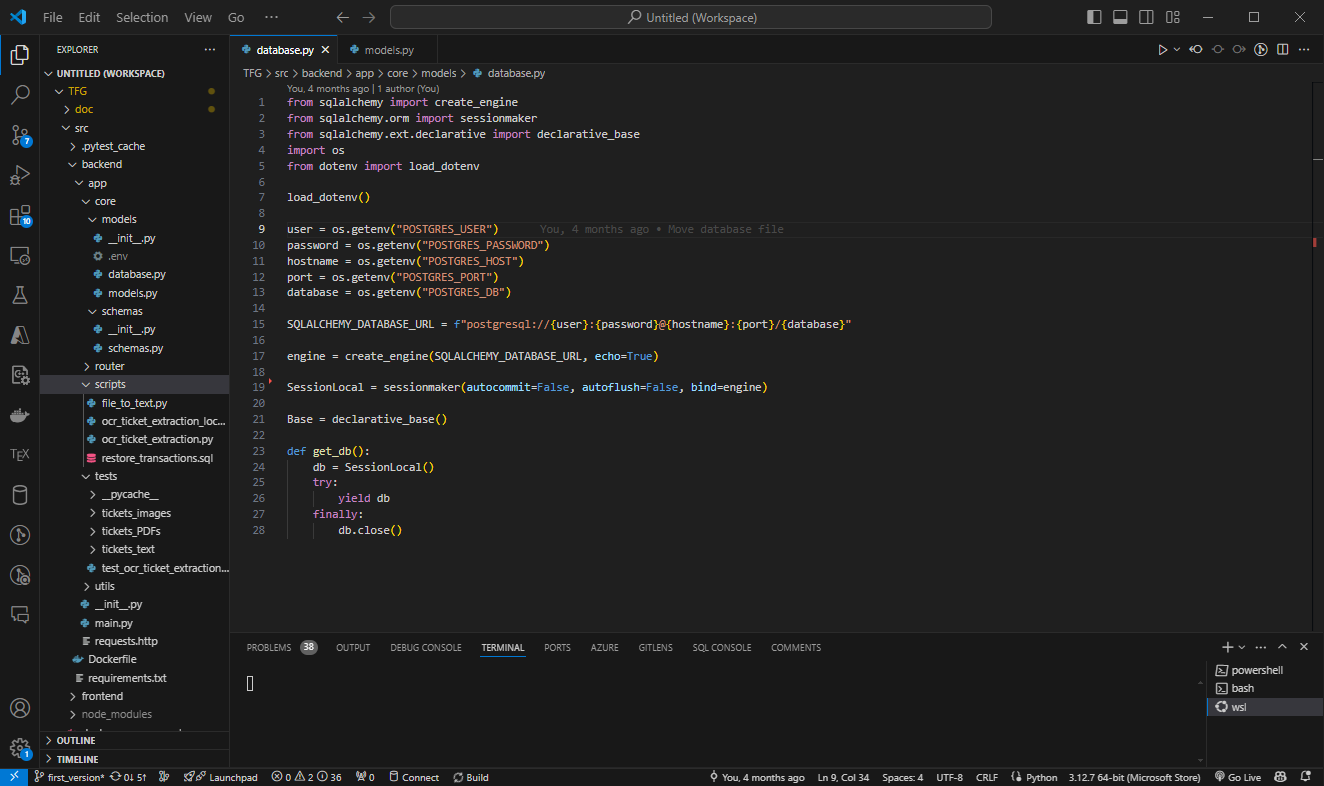
\includegraphics[width=\linewidth]{imagenes/visual_studio_code.png}
    \caption{Visual Studio Code}
    \label{fig:visual_studio_code}
\end{figure}

\subsection{Administrador de base de datos}
Para la gestión de la base de datos se ha utilizado \textbf{DBeaver}\footnote{\url{https://dbeaver.io/}}, una herramienta de código abierto que permite conectar y administrar bases de datos de diferentes tipos, como MySQL, PostgreSQL, SQLite, Oracle, etc. \textit{DBeaver} dispone de una interfaz gráfica intuitiva que facilita, entre otros, la creación y modificación de tablas, la ejecución de consultas SQL, generación de backups.

\begin{figure}[ht!]
    \centering
    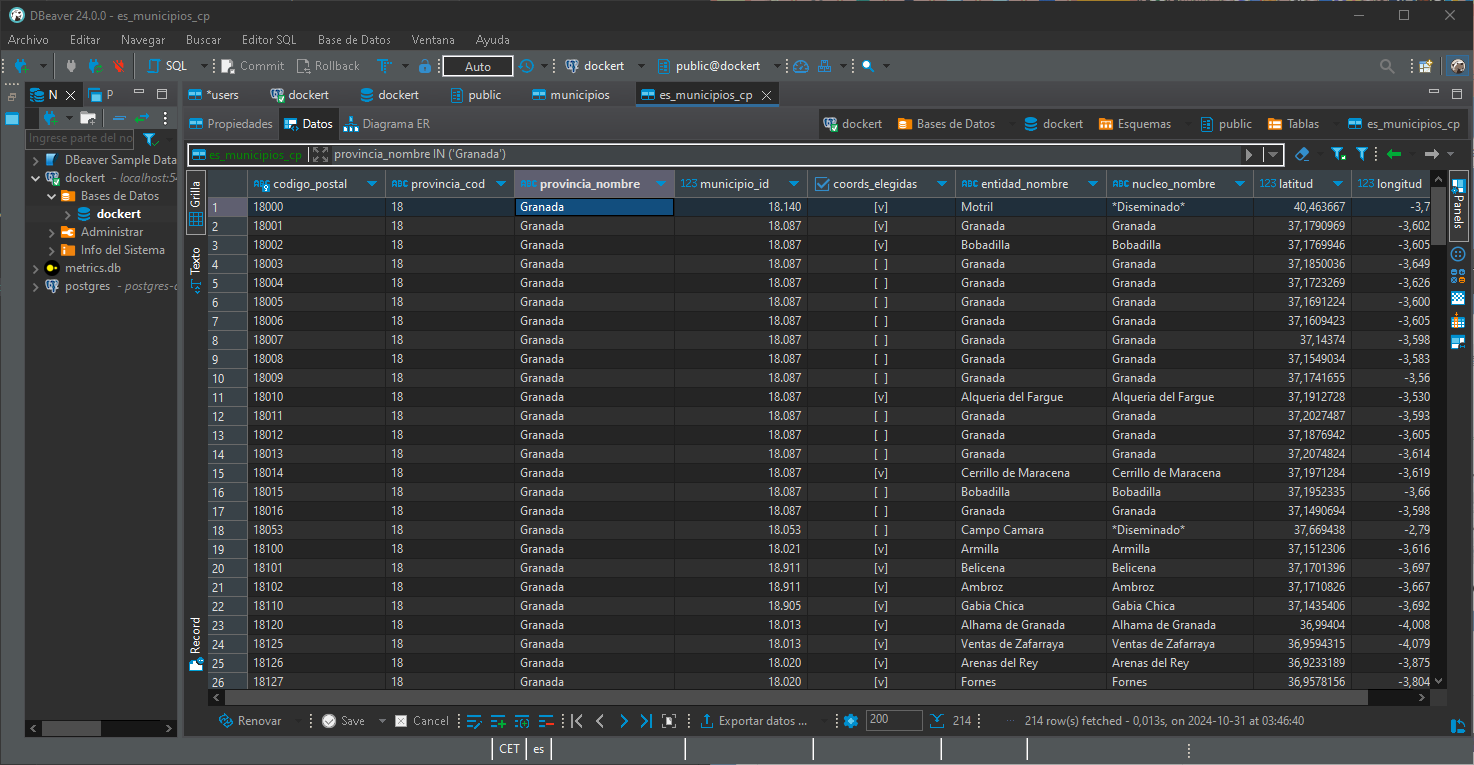
\includegraphics[width=\linewidth]{imagenes/dbeaver.png}
    \caption{Dbeaver}
    \label{fig:dbeaver}
\end{figure}

\subsection{Contenerización}
En el desarrollo de esta aplicación se ha utilizado \textit{Docker}\footnote{\url{https://www.docker.com/}}, una plataforma de código abierto que permite a los desarrolladores empaquetar y distribuir aplicaciones en contenedores. Los contenedores son entornos ligeros y portables que contienen todo lo necesario para ejecutar una aplicación, incluidas las bibliotecas, las dependencias y el código. El uso de \textit{Docker} en este proyecto facilita la creación de entornos de desarrollo y producción consistentes y replicables, lo que garantiza que la aplicación se ejecute de de forma similar en cualquier entorno.
\begin{figure}[ht!]
    \centering
    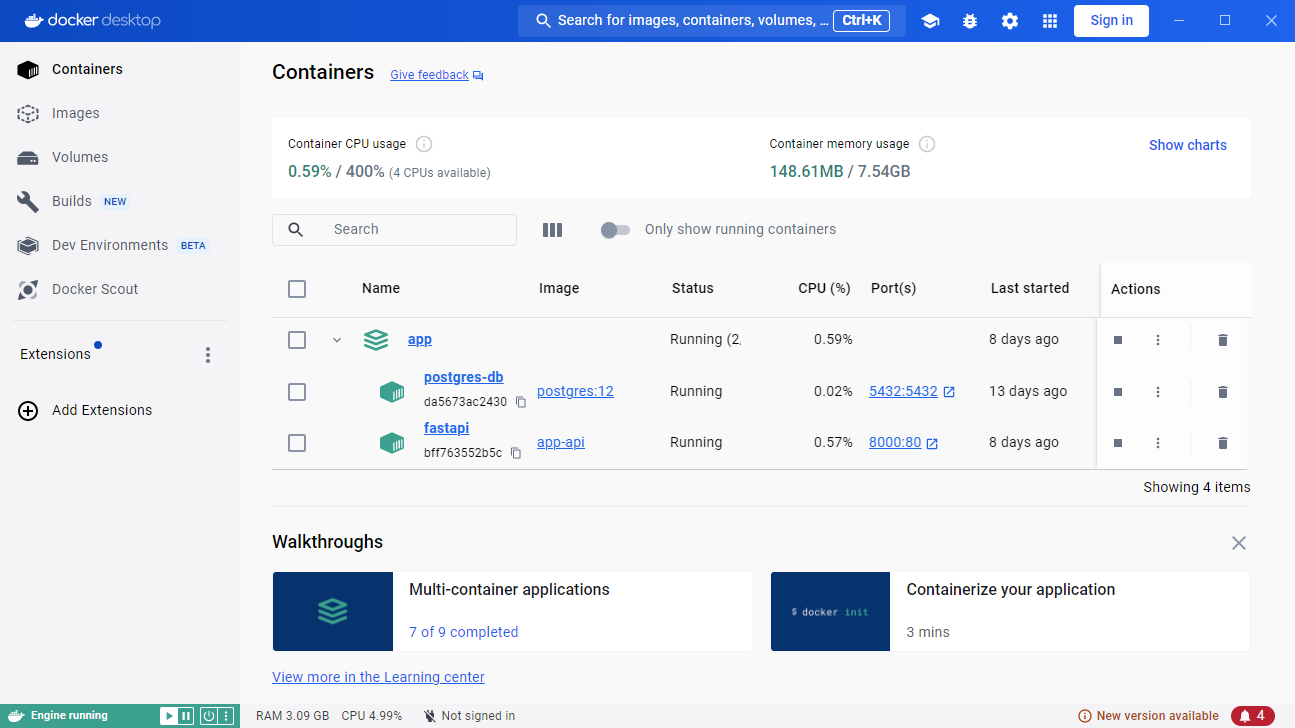
\includegraphics[width=\linewidth]{imagenes/docker.png}
    \caption{Docker}
    \label{fig:docker}
\end{figure}

??? REPETIR CAPTURA CUANDO PASE A DOCKER EL FRONTEND ????


\section{Arquitectura y diseño base. Creación del backend: Milestone 1}
En una arquitectura cliente-servidor (decidida para este proyecto en el comienzo del capítulo anterior), el protocolo HTTP es el estándar de comunicación que el navegador (cliente) utiliza para enviar solicitudes al servidor web y recibir respuestas. Permite al cliente realizar acciones de acuerdo a sus necesidades. Las operaciones HTTP más comunes son las de solicitud de datos (GET), envío de datos al servidor (POST), actualización de datos (PUT) y eliminación (DELETE). 

Para organizar y estandarizar estas interacciones, se emplea una API (Application Programming Interface). Una \textbf{API} es un conjunto de reglas y protocolos que permiten que diferentes aplicaciones se comuniquen entre sí a través de una red. En este proyecto, se utiliza una API REST (Representational State Transfer), que sigue los principios de HTTP, permitiendo que el cliente y el servidor se comuniquen mediante solicitudes HTTP. Una API REST estructura las interacciones en torno a recursos específicos y opera sobre ellos mediante los métodos GET, POST, PUT, y DELETE, brindando una forma eficiente de interactuar con el backend.

La API REST en este proyecto también se beneficia de un \textbf{ORM} (Object-Relational Mapping), que facilita la interacción entre la aplicación y la base de datos. Un ORM permite manipular datos en la base de datos utilizando objetos en el código de la aplicación, evitando escribir directamente consultas SQL. Así, los desarrolladores pueden trabajar con datos a nivel de objetos (como usuarios o transacciones) en lugar de consultas SQL, lo cual simplifica el manejo de datos y mejora la legibilidad del código, a la vez que aporta seguridad al prevenir vulnerabilidades como inyecciones SQL.

Finalmente, la \textbf{base de datos} actúa como fuente de información para la API REST, almacenando todos los datos de la aplicación. La API realiza consultas a la base de datos mediante el ORM, de modo que puede manejar los datos según las solicitudes que recibe del cliente. Esta estructura modular asegura una comunicación fluida y un acceso seguro y eficiente a la información, optimizando la gestión y manipulación de los datos.

Para implementar esta parte que conforma el backend de la aplicación, necesitamos escoger herramientas que se adapten a las necesidades del proyecto.

\subsection{Lenguaje de programación}
\subsubsection{Criterios de búsqueda}
Debe tener soporte para el desarrollo de APIs y para la conexión a la base de datos. Además debe ser compatible con bibliotecas de testing y OCR.

\subsubsection{Criterios de selección}
Para las opciones compatibles con los criterios de búsqueda se eligirá preferentemente aquella donde se cumplan la mayor parte o todos los criterios de selección descritos a continuación.

\begin{itemize}
    \item Conocimiento del lenguaje por parte del desarrollador.
    \item Simplicidad de uso.
    \item Librerías mantenidas o con soporte activo, donde se pueda encontrar información y ejemplos de uso.
    \item Simplicidad en la instalación y uso de OCR.
\end{itemize}

\subsubsection{Opciones compatibles con los criterios de búsqueda}
\begin{itemize}
    \item \textbf{Python}\\
        Conocido por su simplicidad y legibilidad, lo que facilita el desarrollo y mantenimiento del código. Python cuenta con una de las comunidades más grandes, con numerosos recursos, tutoriales y documentación. Respecto al OCR, tiene una ventaja significativa gracias a Pytesseract, una interfaz para Tesseract fácil de usar, con buenos resultados y ampliamente usada para el procesamiento de imágenes. 
    \item \textbf{JavaScript} (Node.js)\\
        En comparación con Python, JavaScript puede tener una curva de aprendizaje más pronunciada y una comunidad de desarrolladores ligeramente más pequeña. El desarrollador tiene menos experiencia desarrollando aplicaciones web en JavaScript que en Python. Por otro lado, aunque puede ser viable su uso, la implementación para OCR es menos eficiente que en Python en términos de rendimiento y facilidad de integración.
    \item \textbf{Java}\\
        La configuración y el desarrollo de una aplicación web en Java pueden requerir más tiempo y esfuerzo en comparación a los anteriores. Aunque el conocimiento del desarrollador en Java es mayor que en Python o JavaScript, de nuevo, aunque dispone de bibliotecas para OCR tiene peor rendimiento que en Python y además suele ser más complicado de configurar.
\end{itemize}

\subsubsection{Opción seleccionada y justificación}
Para el desarrollo de la aplicación se ha seleccionado \textbf{Python} como lenguaje de programación. Python cumple con todos los criterios de búsqueda y ofrece una amplia gama de bibliotecas y herramientas para el desarrollo de APIs, la conexión a la base de datos y otras funcionalidades necesarias para este proyecto. A pesar de no ser el lenguaje de programación más conocido por el programador, su simplicidad y el mejor rendimiento para OCR lo pone por encima del resto.

??? EXPLICAR AQUÍ QUE QUIZÁS HUBIERA SIDO MEJOR NODE PORQUE LO USO LUEGO EN EL FRONTEND ASÍ QUE HUBIERA SIDO MÁS COHERENTE ???

\subsection{Framework de backend}
\subsubsection{Criterios de búsqueda}
Debe estar optimizado para crear APIs de forma rápida y eficiente.
Debe ofrecer compatibilidad con el lenguaje de programación elegido (Python). También debe contar con integración de ORMs.

\subsubsection{Criterios de selección}
\begin{itemize}
    \item Se valorará positivamente la facilidad para documentar y si dispone de un entorno para pruebas.
    \item Se prioriza un framework que gestione eficientemente las solicitudes HTTP, con soporte para programación asíncrona, de forma que se optimice el rendimiento a la hora de atender gran número de solicitudes de forma simultánea. ?????? Sí, pero tengo que hacer las pruebas de benchamark al final (mirar mis notas) para demostrarlo. ?????
\end{itemize}

\subsubsection{Opciones compatibles con los criterios de búsqueda}
\begin{itemize}
    \item \textbf{Django}\\
        Permite crear documentación pero no se genera de forma automática, lo que requiere un esfuerzo manual mayor. 
        Cuenta con bibliotecas y soporte para testing. No es totalmente asíncrono, ofrece soporte asíncrono parcial.
    \item \textbf{Flask}\\
        Un framework ligero y modular, pero sin soporte asíncrono nativo (desde Flask 2.0 se incluye con limitaciones) y sin generación automática de documentación. Este framework también cuenta con bibliotecas y soporte para testing.
    \item \textbf{FastAPI}\\
        Fue diseñado específicamente para la creación de APIs de alto rendimiento y maneja solicitudes HTTP de manera eficiente al soportar asincronía nativa.
        Genera documentación de forma automática, lo que simplifica la validación y pruebas de los endpoints.
\end{itemize}

\subsubsection{Opción seleccionada y justificación}
\textbf{FastAPI} se eligió por la generación automática de documentación que además permite realizar pruebas de los endpoints. También por su excelente soporte para programación asíncrona, que aunque en el inicio del proyecto no va a marcar diferencias grandes, en caso de que la aplicación crezca y gestione un número elevado de usuarios, la programación asíncrona ayuda a mejorar la eficiencia. Esto permite a la aplicación gestionar múltiples solicitudes simultáneas sin degradar el rendimiento.


\subsection{Base de datos}
Las bases de datos relacionales son mejores para datos estructurados y consistentes, mientras que las bases de datos no relacionales son más adecuadas para datos que cambian en estructura o en aplicaciones que requieren escalabilidad horizontal. 

En una aplicación de gestión financiera como la de este proyecto, se opta por una base de datos relacional, ya que siendo los datos estructurados, estas permiten establecer relaciones y restricciones entre tablas, lo cual asegura que los datos se mantengan consistentes y libres de errores.

\subsubsection{Criterios de búsqueda}
Debe ser una base de datos relacional. Deben existir bibliotecas de Python que permitan la conexión con la base de datos, y ser escalable y adecuada para entornos de producción.

% Para esta aplicación de gestión bancaria, se prefieren bases de datos que ofrezcan soporte para consultas SQL avanzadas, gestión segura de transacciones y alta concurrencia. Es crucial que la base de datos sea confiable, escalable y adecuada para entornos de producción con múltiples usuarios.

\subsubsection{Criterios de selección}
\begin{itemize}
    \item La base de datos debe tener soporte para consultas complejas y relaciones entre tablas. 
    \item Su manejo eficiente de concurrencia y alta escalabilidad. Además, como puede llegar a usarse por múltiples usuarios que accedan a la base de datos simultáneamente, es importante que sea robusta y segura.
    \item  Es importante que cuente con una comunidad activa y amplia documentación.
\end{itemize}

\subsubsection{Opciones compatibles con los criterios de búsqueda}
\begin{itemize}
    \item \textbf{PostgreSQL}\\
        Cuenta con una extensa comunidad y documentación.
        PostgreSQL tiene un motor de optimización de consultas avanzado y es muy eficiente en la ejecución de consultas complejas que involucran múltiples tablas y condiciones. PostgreSQL tiene un excelente soporte para integridad referencial y permite definir restricciones complejas entre tablas.
    \item \textbf{MySQL}\\
        Carece de algunas funcionalidades avanzadas necesarias para consultas y transacciones complejas. Aunque es una buena opción para aplicaciones de lectura intensiva, su soporte para concurrencia es limitado en comparación con PostgreSQL.

        Si bien MySQL también permite definir relaciones, PostgreSQL maneja mejor las relaciones y restricciones, lo cual es crucial en una aplicación donde los errores de integridad podrían causar inconsistencias en los saldos o movimientos financieros.
        
    \item \textbf{SQLite}\\
        Ideal para prototipado y desarrollo local, pero no es adecuado para producción debido a su falta de soporte para concurrencia a gran escala. Debido a que es ligero y fácil de usar no tiene una documentación tan extensa como los anteriores.
\end{itemize}
\subsubsection{Opción seleccionada y justificación}
\textbf{PostgreSQL} es la opción más robusta, con soporte para transacciones avanzadas, escalabilidad y flexibilidad en el manejo de datos complejos, lo que garantiza un rendimiento confiable.

\subsection{ORM}
\subsubsection{Criterios de búsqueda}
El ORM debe ser compatible con Python, el framework FastAPI y la base de datos relacional PostgreSQL.

\subsubsection{Criterios de selección}
\begin{itemize}
    \item Debe tener documentación extensa y comunidades activas para resolver problemas y dudas. Es fundamental que el ORM se integre bien con FastAPI y PostgreSQL, manteniendo un flujo de datos eficiente y seguro entre la API y la base de datos.
\end{itemize}

\subsubsection{Opciones compatibles con los criterios de búsqueda}
\begin{itemize}
    \item \textbf{Django ORM}\\
        Eficiente y fácil de usar en el contexto de proyectos Django, pero tiene una integración limitada con FastAPI y depende fuertemente del framework Django, lo que reduce su flexibilidad en proyectos que no utilicen Django directamente. Su documentación es extensa y cuenta con una comunidad activa.
    \item \textbf{SQLAlchemy}\\
        Ofrece una gran flexibilidad y control sobre las consultas, con soporte para PostgreSQL y buena compatibilidad con FastAPI. Es ampliamente usado en la comunidad de Python y es una opción madura y ampliamente documentada. Gracias a su uso extendido cuenta con una comunidad activa.
    \item \textbf{Tortoise ORM}\\
        Un ORM asíncrono que se adapta bien a FastAPI y proporciona un rendimiento eficiente en aplicaciones asincrónicas. Sin embargo, tiene una documentación menos extensa que SQLAlchemy y una comunidad más pequeña que va creciendo.
\end{itemize}

\subsubsection{Opción seleccionada y justificación}
\textbf{SQLAlchemy} ha sido seleccionado por su flexibilidad, amplia documentación y compatibilidad con PostgreSQL y FastAPI. Su robustez para manejar consultas complejas y su alta compatibilidad con otras herramientas de la comunidad Python lo hacen una opción ideal para la aplicación, permitiendo un desarrollo escalable.


\subsection{Implementación del backend}
A continuación se describen los pasos seguidos para la implementación del backend de la aplicación utilizando las herramientas seleccionadas.

La implementación se hizo usando Docker, ya que facilita la creación de entornos de desarrollo y producción consistentes, replicables y más seguros, quedando dos servicios interrelacionados: una API desarrollada con FastAPI y una base de datos PostgreSQL; cada uno con una configuración concreta. 

Se creó un contenedor a partir de la imagen oficial de PostgreSQL (versión 12), el sistema de gestión de bases de datos relacional elegido.

FastAPI no se instaló a partir de una imagen existente como tal, sino que se creó una personalizada a partir de una imagen ya existente de Python en su versión 3.10, el resto de configuraciones para utilizar FastAPI se extraen del archivo \textit{Dockerfile} creado en los ficheros del backend de la aplicación. Este archivo contiene las instrucciones para instalar las dependencias necesarias y configurar el entorno de ejecución de la aplicación dentro del entorno completo de Python que proporciona la imagen base. 

\begin{itemize}
    \item \textbf{Modelo de la base de datos}\\
        Se crearon tablas siguiendo el modelo del diagrama UML creado en la fase de diseño. Dichas tablas se crearon como clases en Python utilizando SQLAlchemy, lo que permitió definir las relaciones entre tablas para garantizar la integridad de los datos y se definieron restricciones para asegurar la coherencia de la información. Las clases se encargan de mapear los objetos de Python a las tablas de la base de datos, facilitando la interacción con la base de datos y la manipulación de los mismos.

    \item \textbf{Esquemas de validación}\\
        Aprovechando la integración de FastAPI con Pydantic, se crearon esquemas de validación para cada entidad, lo que facilitó la validación de los datos en las solicitudes HTTP, aportando seguridad y consistencia a la aplicación.

    \item \textbf{Endpoints}\\
        Se crearon los endpoints de la API REST utilizando FastAPI, definiendo las rutas y los métodos HTTP que utilizar para interactuar con la API. Para ello se implementaron las operaciones CRUD \textit{(Create, Read, Update, Delete)} para cada entidad de la base de datos, lo que permitió realizar las operaciones básicas de gestión de datos.

    \item \textbf{Persistencia}\\
        Con una configuración simple de volúmenes en Docker, se garantizó la persistencia de los datos en la base de datos PostgreSQL. Con la definición del volumen persistente, los datos se almacenan fuera del contenedor, lo que asegura que estos se mantengan incluso después de reiniciar el contenedor o eliminarlo.

    \item \textbf{Pruebas}\\
        Se revisó con DBeaver la correcta creación y estructura de las tablas en la base de datos.
        Desde la documentación generada automáticamente en FastAPI, se realizaron varios tipos de pruebas básicas para verificar el funcionamiento correcto de los endpoints y la interacción con la base de datos. Entre ellas se realizaron algunas pruebas de conectividad a la base de datos (comprobando que se podía acceder a los datos), pruebas CRUD para examinar las operaciones de creación, lectura, actualización y eliminación de cada entidad y pruebas de validación de datos para comprobar que las restricciones definidas en los esquemas de validación son detectadas correctamente.
\end{itemize}

\subsubsection{Componente backend}
Finalmente, se obtuvo un componente backend funcional que proporciona una API REST para la gestión de datos de la aplicación. Este componente se encarga de la gestión de la base de datos y la validación de los mismos. Permite la interacción con el frontend cuyo desarrollo se describe en el siguiente milestone \ref{cap:milestone2}. En la Figura \ref{fig:endpoints} se muestran algunos de los endpoints creados, concretamente los relacionados con las operaciones con las entidades que representan a las subcategorías, las transacciones de forma general y más concretamente las transacciones de tipo \textit{ingreso}. La documentación de la API generada automáticamente por FastAPI permite visualizar estos endpoints y realizar las pruebas mencionadas de forma sencilla.

\begin{figure}[ht!]
    \centering
    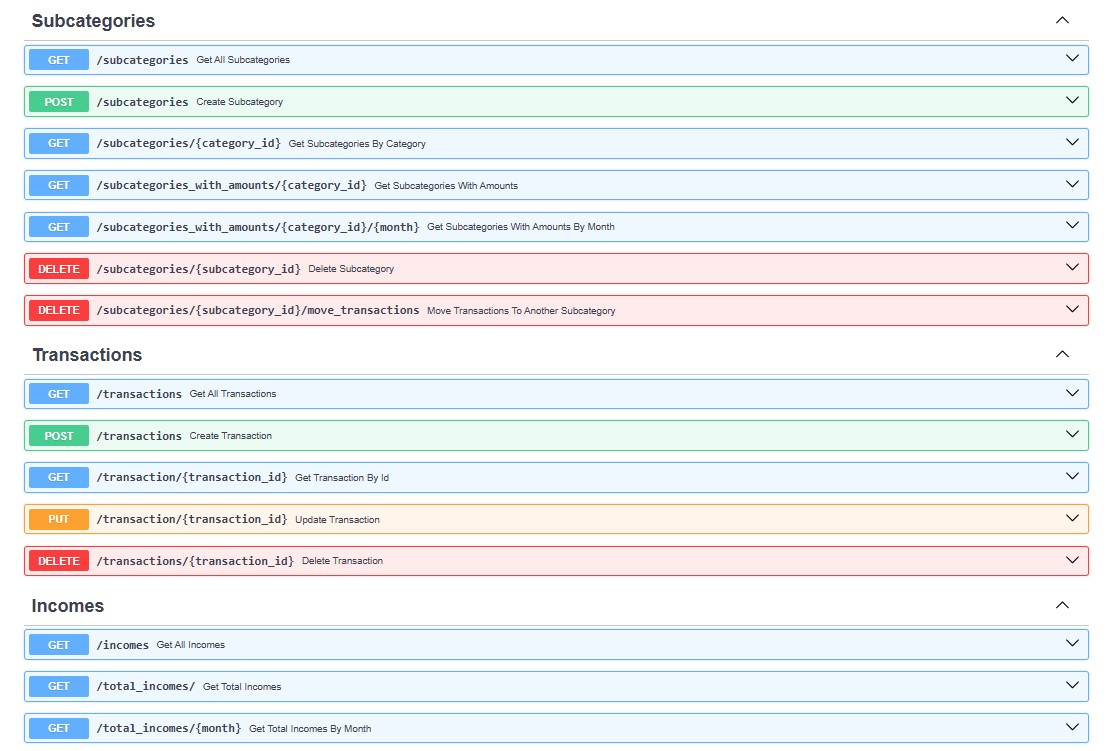
\includegraphics[width=\linewidth]{imagenes/endpoints.jpg}
    \caption{Endpoints de la API REST}
    \label{fig:endpoints}
\end{figure}


\section{Creación de la interfaz de usuario: Milestone 2}\label{cap:milestone2}
El frontend es la parte de la aplicación que permite al usuario interactuar con la aplicación. Es el elemento ejecutor de las acciones que el usuario desea realizar. Recibe las solicitudes del usuario, las envía al backend (mediante la API) para que sean procesadas y las devuelve al frontend para que el usuario visualice los resultados.

Esta implementación del cliente debe ser capaz de mostrar la información de forma clara y facilitar al usuario una interacción intuitiva con la aplicación. Para ello, se ha seguido el diseño de la interfaz de usuario definido en el la sección \ref{sec:diseno_interfaz_usuario}.


\subsection{Framework o biblioteca para frontend}
Para el desarrollo del frontend de la aplicación se debe elegir un framework o biblioteca que permita desarrollar y mantener interfaces de usuario de forma eficiente y escalable. 

\subsubsection{Criterios de búsqueda}
El framework o biblioteca debe ser compatible con FastAPI. Debe tener soporte para el desarrollo de componentes reutilizables, de modo que se agilice el desarrollo y mantenimiento de la interfaz de usuario. 

\subsubsection{Criterios de selección}
\begin{itemize}
    \item Debe tener una curva de aprendizaje moderada.
    \item Debe tener una amplia base de usuarios y buena documentación para facilitar el aprendizaje y la resolución de problemas.
    \item Debe ser adecuado para añadir futuras funcionalidades o integración de bibliotecas.
    \item Se valorará el interés del desarrollador en la herramienta, ya que esto puede influir en la eficiencia del desarrollo.
\end{itemize}

\subsubsection{Opciones compatibles con los criterios de búsqueda}
\begin{itemize}
    \item \textbf{React}\\
        Es una biblioteca de JavaScript enfocada en crear interfaces de usuario usando componentes reutilizables. Por su popularidad, cuenta con una extensa comunidad y herramientas.
    \item \textbf{Vue}\\
        Puede usarse como biblioteca o como un framework completo. Es ligero y flexible, al ser modular permite añadir solo las funcionalidades necesarias. Es menos popular que React, pero tiene una comunidad activa y una curva de aprendizaje más suave.
    \item \textbf{Angular}\\
        Es un framework de frontend completo que facilita el desarrollo de aplicaciones web complejas y escalables. Angular tienen un proceso de aprendizaje más complejo que React y Vue, pero ofrece un enfoque en la estructura y modularidad, además de un conjunto de herramientas muy completo.
\end{itemize}

\subsubsection{Opción seleccionada y justificación}
Dado que todas las tres herramientas cumplen los criterios de selección mínimos, se ha elegido \textbf{React} porque, a pesar de no tener la menor curva de aprendizaje, es la herramienta que más interés despierta en el desarrollador.

\subsection{Herramientas de desarrollo en React}
Se han usado ciertas herramientas que facilitan y optimizan el proceso de desarrollo en React.

React está basado en \textbf{JavaScript}, que es el lenguaje que se encarga de la interacción con el DOM\footnote{ El DOM \textit{(Document Object Model)} es una interfaz de programación para documentos HTML y XML. Define la estructura lógica de los documentos y la forma en que se accede a ellos y se modifican.}, controla el comportamiento de los componentes y permite escribir en \textbf{JSX},\footnote{JSX es una extensión de JavaScript que permite incluir HTML dentro del código JavaScript.} que se utiliza en React para construir componentes interactivos y reutilizables.

El primer paso, por tanto, será instalar \textbf{Node.js}, que incluye \textbf{NPM} \textit{(Node Package Manager)}, un gestor de paquetes de JavaScript que permite instalar y gestionar  fácilmente las dependencias que se necesitan en el proyecto

Para agilizar el desarrollo se ha usado la herramienta de compilación \textbf{Vite}. Entre otros, mejora el tiempo de inicio del servidor, hace una traducción rápida de JSX a Javascript y optimiza la carga del código en producción.

\subsection{Implementación del frontend}
La aplicación presenta varias vistas con estructura similar pero diferente información, por ello se ha priorizado la reutilización de componentes todo lo posible, para facilitar el mantenimiento, la escalabilidad y la coherencia visual.

El diseño de componentes se ha ayudado de herramientas como \textbf{Tailwind CSS} junto con \textbf{DaisyUI}, que permiten usar componentes preconstruidos y estilos atractivos de forma rápida y sencilla. Y las bibliotecas \textbf{Heroicons} y \textbf{Headless UI}, que ofrecen iconos y componentes fáciles de incorporar.


\begin{itemize}
    \item \textbf{Componentes reutilizables}
        Se han creado componentes reutilizables para elementos comunes en la aplicación, como botones, formularios, etc. Esto permite mantener la coherencia visual y facilita la creación de nuevas vistas.
    \item \textbf{Rutas}
        Se han definido las rutas de la aplicación, que permiten al usuario navegar entre las diferentes vistas. Se han creado rutas para cada vista y se han definido las acciones que se deben realizar al acceder a cada ruta.
    \item \textbf{Interacción con la API}
        La forma en que el frontend es capaz de realizar solicitudes es con la biblioteca \textbf{Axios}, que permite realizar solicitudes HTTP de forma sencilla y eficiente. Axios se encarga de enviar las solicitudes al backend con los datos necesarios y de procesar las respuestas, lo que facilita la interacción con la API y la manipulación de los datos. Las solicitudes se generan por la interacción del usuario con la interfaz, por ejemplo, al hacer clic en un botón o al enviar un formulario.
    \item \textbf{Pruebas}
        Se han realizado pruebas para verificar el correcto funcionamiento de los componentes y la interacción con la API. Se han comprobado manualmente las rutas, la interacción con los componentes y la visualización de la información.
\end{itemize}


\subsection{Operaciones desde la interfaz de usuario}
Entre las operaciones implementadas para que el usuario pueda ejecutarlas en la aplicación web, encontramos:

\begin{itemize}
    \item \textbf{Creación}
        El usuario puede crear nuevos elementos, como transacciones, categorías de gasto, objetivos de ahorro, etc. Para ello, la aplicación muestra un formulario con los campos necesarios para la creación del elemento, el usuario debe rellenar los campos y enviar el formulario para que la información se almacene en la base de datos.        
    \item \textbf{Modificación}
        Del mismo modo, por medio de un formulario el usuario puede modificar los elementos ya existentes. La aplicación muestra los datos actuales del elemento y permite al usuario modificarlos y guardar los cambios en la base de datos.
    \item \textbf{Eliminación}
        La aplicación permite al usuario eliminar todos los elementos que él mismo ha creado. Al hacer clic en el botón de eliminar, la aplicación muestra una confirmación y, si el usuario confirma la eliminación, se elimina el elemento de la base de datos.
    \item \textbf{Visualización de transacciones}
        La aplicación muestra al usuario la información de las transacciones almacenadas en la base de datos, permitiendo al usuario ver sus movimientos financieros y analizar su historial.        
\end{itemize}

\subsubsection{Componente frontend}
Finalmente, se obtuvo un componente frontend funcional que se encarga de mostrar la información de forma clara y organizada, y permite al usuario interactuar con la aplicación. Los elementos que conforman el frontend permiten al usuario navegar entre las diferentes vistas y realizar las operaciones descritas anteriormente. En la Figura \ref{fig:componentes_frontend} se muestra un esquema de los componentes principales de la aplicación. En las figuras \ref{fig:ingreso_form} y \ref{fig:ingreso_lista} se pueden ver dos elementos del frontend que interactúan con los endpoints de las operaciones de tipo \textit{ingreso} mostradas en el backend.

\begin{figure}[ht!]
    \centering
    \begin{minipage}{0.45\textwidth}
        \centering
        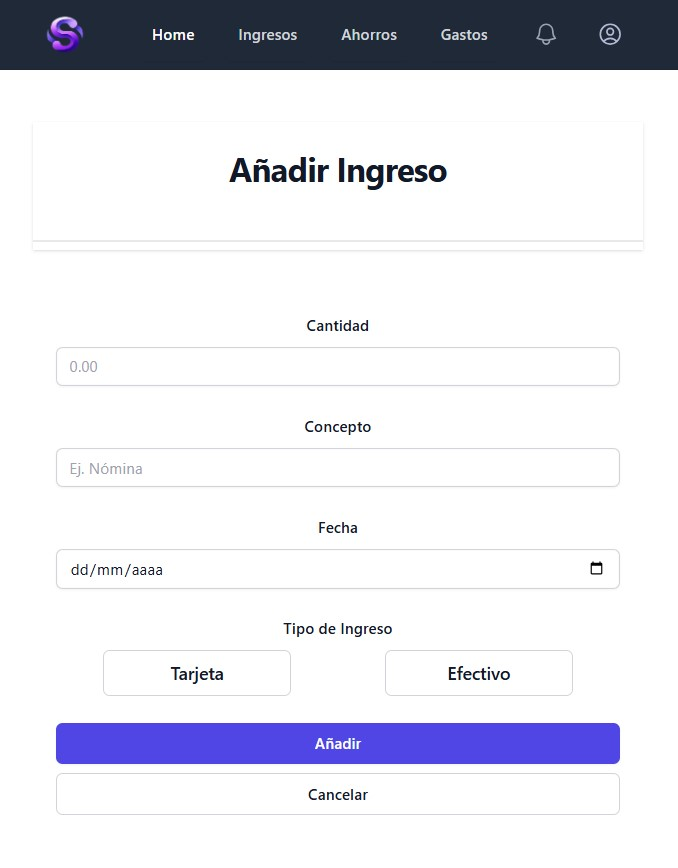
\includegraphics[height = 70mm]{imagenes/ingreso_form.jpg}
        \caption{Elemento frontend para añadir un ingreso}
        \label{fig:ingreso_form}
    \end{minipage}\hfill
    \begin{minipage}{0.45\textwidth}
        \centering
        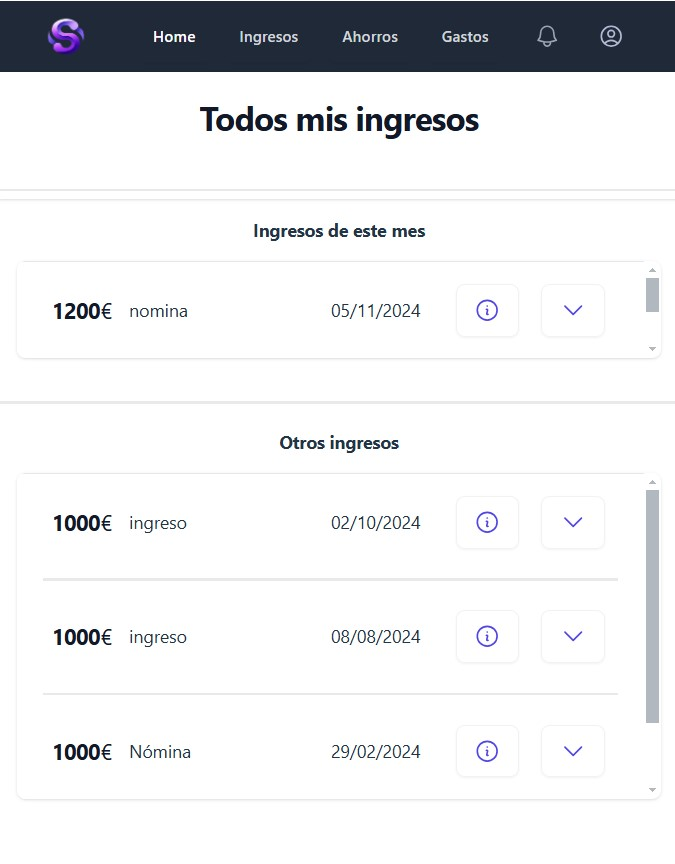
\includegraphics[height = 70mm]{imagenes/ingreso_lista.jpg}
        \caption{Elemento frontend para visualizar la lista de ingresos}
        \label{fig:ingreso_lista}
    \end{minipage}
\end{figure}


\subsubsection{Vistas de la aplicación}
Indagando más en la visualización de transacciones, se han creado diferentes vistas para mostrar la información de las transacciones de forma clara y organizada. Se han creado vistas para mostrar los gastos mensuales por categorías, los ahorros por objetivos, etc. Cada vista muestra la información de forma simple, lo que permite al usuario analizar sus gastos y tomar decisiones informadas sobre su economía.


La navegación entre las diferentes vistas de la aplicación se ha implementado con \textbf{React Router}, para definir rutas y acciones a realizar al acceder a cada una. Se han creado rutas para cada vista, y se ha definido cada vista como un componente de React, con lo que hemos construido una aplicación de una sola página (SPA, \textit{Single Page Application}) que permite al usuario navegar entre las diferentes vistas sin necesidad de recargar la página en el navegador. 


Entre las diferentes vistas, podemos agruparlas por la funcionalidad de la que se encargan para entender mejor su implementación. Por ejemplo, la modificación o creación de transacciones se hace por medio de formularios, la eliminación suele hacerse con un botón incluido en la visualización del elemento concreto, etc. Cada grupo de vistas está formado por componentes comunes que se reutilizan y por componentes específicos que se encargan de mostrar la información que diferencia una vista de la otra con la que comparte elementos. 


Las principales vistas donde se muestra la información que dará valor a los datos almacenados del usuario se describen a continuación. En la Figura \ref{fig:componentes_frontend} se muestran estas vistas principales y la navegabilidad entre ellas, mostrando su estructura de componentes. Cada caja corresponde a un componente implementado en React.

\begin{itemize}
    \item \textbf{Vista de inicio (\textit{HomeView}).} Muestra por separado la suma total de ingresos, gastos y ahorros del usuario en el mes actual. Se corresponde con el concepto de monedero o cartera, donde el usuario puede ver de un vistazo su situación financiera del mes.
    \item \textbf{Vista de gastos mensuales (\textit{ExpensesOverviewView}).} Muestra la cantidad total de gastos del usuario en el mes actual. Desglosa también la cantidad total entre las diferentes categorías de gasto y mostrando el total acumulado por cada una de ellas y mostrando cuánto queda para llegar al límite del presupuesto establecido.
    \item \textbf{Vista de ahorros (\textit{SavingsOverviewView}).} Muestra la cantidad total apartada como ahorro del usuario en el mes actual. Desglosa también la cantidad total entre los diferentes objetivos de ahorro y muestra el progreso de cada uno de ellos. En este caso, aunque la cifra de resumen total muestra lo ahorrado solo en el mes actual, los objetivos de ahorro se consideran a largo plazo, por lo que se muestra también el total ahorrado hasta el momento para cada uno (incluyendo las aportaciones de meses anteriores).
    \item \textbf{Vista de categoría de gasto (\textit{CategoryView}).} Muestra la cantidad total de gastos del usuario en la categoría seleccionada durante el mes actual, incluyendo los movimientos realizados en cualquier subcategoría perteneciente a la categoría seleccionada.
    \item \textbf{Vista de objetivo de ahorro (\textit{SavingsGoalView}).} Muestra la cantidad total ahorrada por el usuario en el objetivo de ahorro seleccionado durante el mes actual y el total desde que comenzó a ahorrar para dicho objetivo, incluyendo todos los movimientos de ahorro realizados. Muestra también una barra de progreso, que indica cuánto queda para alcanzarlo. 
    \item \textbf{Las vistas de trasacciones (\textit{TransactionsView}).} muestran para el elemento que se consultada todas las transacciones separadas en dos paneles: transacciones del mes actual y transacciones de meses anteriores.
\end{itemize}

\begin{figure}[ht!]
    \centering
    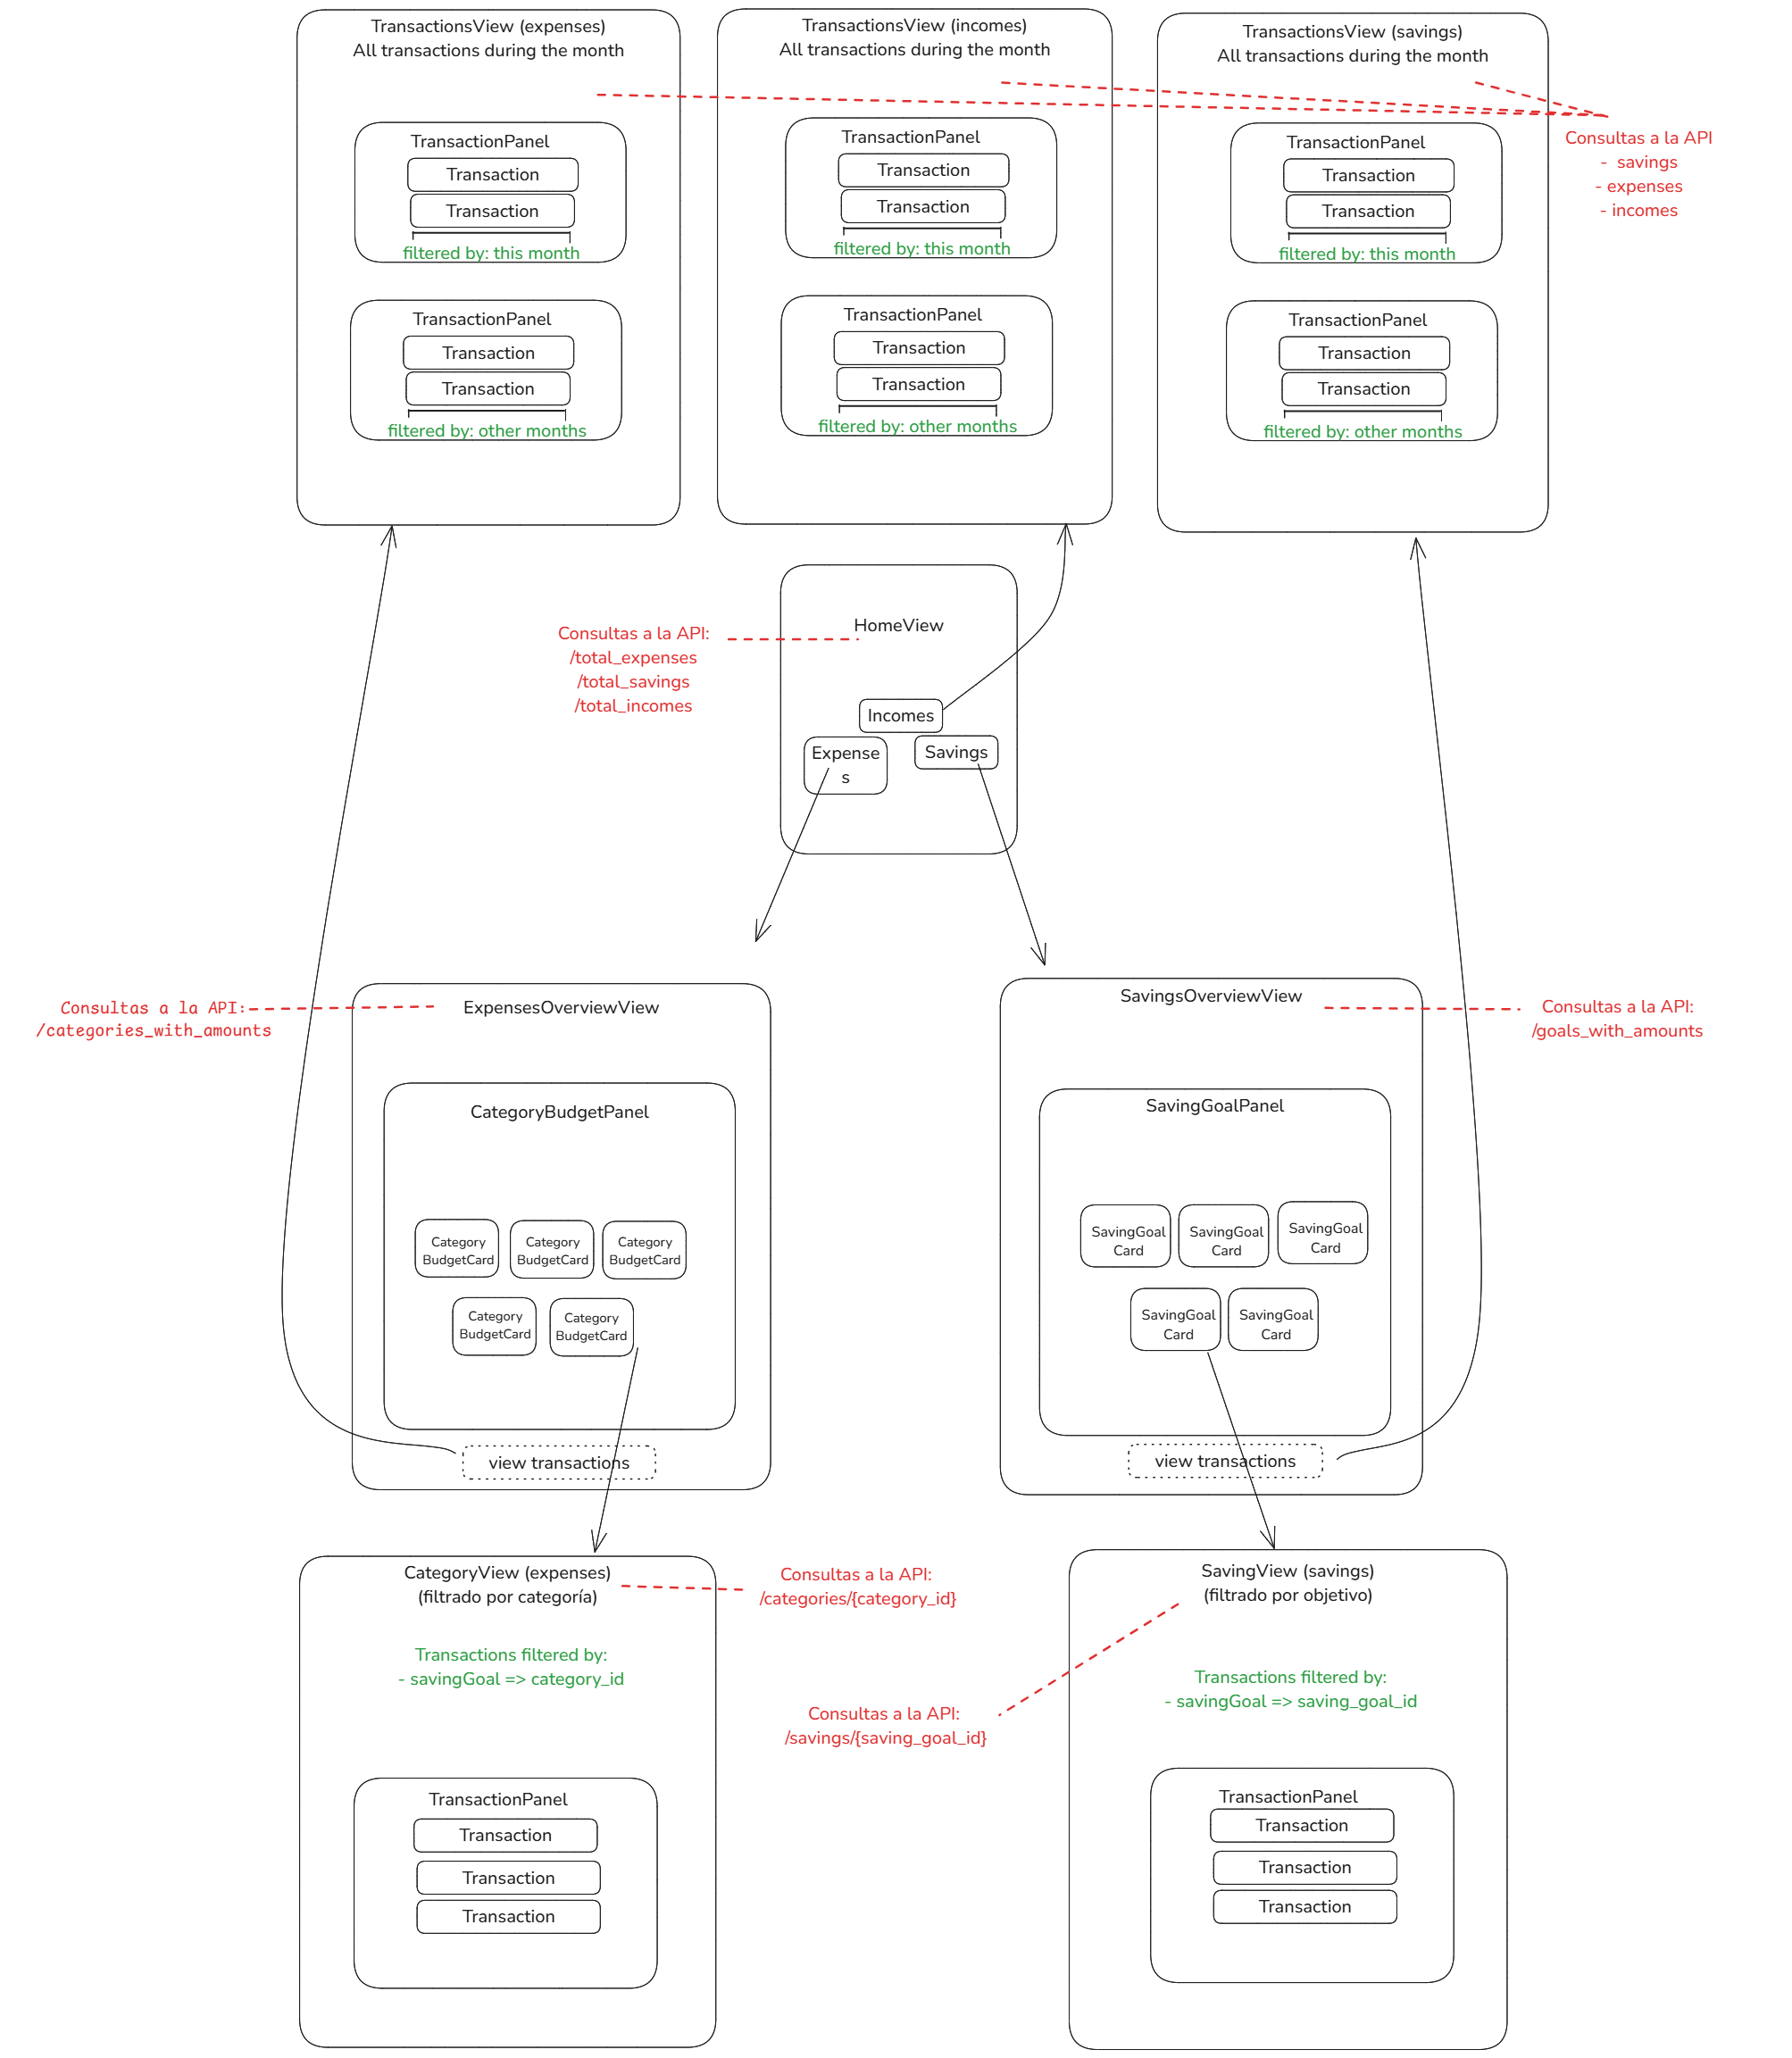
\includegraphics[width=\linewidth]{imagenes/componentes-frontend.png}
    \caption{Vistas principales de la aplicación}
    \label{fig:componentes_frontend}
\end{figure}



\section{Generación de gráficos y resúmenes: Milestone 3}\label{cap:milestone3}
En la implementación del frontend, con el fin de facilitar el mantenimiento y la escalabilidad del código, se pueden crear componentes de tipo \textit{smart} y componentes de tipo \textit{dumb}. Los componentes \textit{smart} son aquellos que tienen la lógica de negocio y se encargan de realizar las solicitudes al backend. Por otro lado, los componentes \textit{dumb} son componentes más simples que se encargan de mostrar la información, con los que actúa directamente el usuario. De esta manera, se sigue el principio de responsabilidad única por cada componente. En el desarrollo se ha seguido esta recomendación, aunque no es una regla estricta, por lo que la estructura del código puede variar dependiendo de las necesidades específicas en aplicación o las preferencias del desarrollador.

En este milestone se implementan las funcionalidades de la aplicación que permiten visualizar gráficos y resúmenes de los datos almacenados en la base de datos.

\subsection{Gráficos y resúmenes}
Tomando de ejemplo la vista de gastos, se describe a continuación cómo se ha implementado la funcionalidad para incluir gráficos y resúmenes de gastos en la aplicación. Se refleja claramente la estructura de componentes \textit{smart} y \textit{dumb}, ya que los dos componentes reciben la información desde el componente de vista de gastos (que es quien realiza la petición con Axios), por lo que se encargan exclusivamente de la representación de la información\cite{khan2023reactjs}. En la Figura \ref{fig:componentes_graficos_resumenes} se puede ver qué parte supone cada componente en la vista de ahorros.

\begin{figure}[ht!]
    \centering
    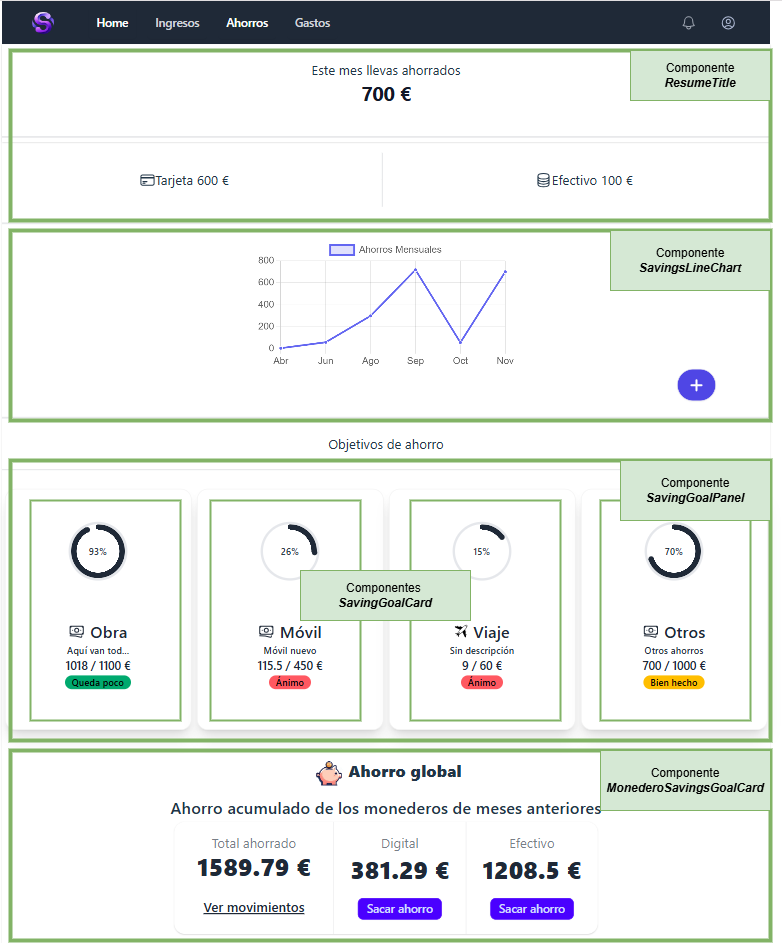
\includegraphics[width=\linewidth]{imagenes/componente-graficos-resumenes.drawio.png}
    \caption{Componentes de gráficos y resúmenes en la vista de ahorros}
    \label{fig:componentes_graficos_resumenes}
\end{figure}


\subsubsection{Resúmenes}
Los resúmenes creados tienen como objetivo mostrar al usuario de forma clara y concisa la información relevante de los datos del mes. Se crearon diferentes componentes para mostrar los resúmenes de ingresos, gastos y ahorros, que se reutilizan en las diferentes vistas de la aplicación con los datos que el usuario consulte. Usando de referencia los componentes en la vista de ahorros (que es la más completa) se describen a continuación los componentes principales de resumen que se han implementado.


El resumen general debe mostrar la cifra de dinero correspondiente al total de sumar cada transacción del mes que coincida con el tipo de movimiento consultado. Debe incluir el desglose de dicha cantidad en dos partes: el total en efectivo y el total en digital.

Los resúmenes que aparecen en la parte superior de las vista de ahorro (componente \textit{ResumeTitle} en la imagen \ref{fig:componentes_graficos_resumenes}), se han creado añadiendo endpoints que, partiendo de las transacciones almacenadas en la base de datos, suman la cantidad del tipo de transacción (en este caso ahorro) y método de pago (efectivo o digital) que se quiere mostrar, filtrando la búsqueda para un usuario y mes determinados. Después se creó un componente en React para mostrar la información a partir del resultado de llamar a dicho enpoint.

\begin{lstlisting}[language=Python, caption=Componente de React para el resumen de gastos]
    import { LoadingDots } from "./LoadingDots";

    export function ResumeTitle({title, amount, card, cash, currency}) {
        return (
            <div>
                <header className="bg-white shadow">
                <div className="mx-auto max-w-7xl px-4 py-6 sm:px-6 lg:px-8">
                    <p>{title}</p>
                    {amount !== "loading" ? (
                        <h1 className="text-3xl font-bold tracking-tight text-gray-900">{amount} {currency}</h1>
                    ) : (
                        <LoadingDots />
                    )}
                </div>
                <div className="divider"></div>
                </header>
    
                <div className="panel flex w-full justify-evenly">
                    <div className="card flex h-20 flex-row place-items-center">
                        <svg> IconoTarjeta </svg>
                        {card !== "loading" ? (
                            <p>Tarjeta {card} {currency}</p>
                        ) : (
                            <p>Tarjeta <LoadingDots /></p>
                        )}
                        
                    </div>
                    <div className="divider divider-horizontal"></div>
                    <div className="card flex h-20 flex-row place-items-center">
                        <svg> IconoEfectivo </svg>
                        {cash !== "loading" ? (
                            <p>Efectivo {cash} {currency}</p>
                        ) : (
                            <p>Efectivo <LoadingDots /></p>
                        )}
                    </div>
                </div>
            </div>  
        );
    };
\end{lstlisting}

Para el resto de resúmenes se ha seguido un proceso similar. 

\begin{itemize}
    \item Resumen de progreso en los objetivos de ahorro (componente \textit{SavingGoalPanel} en la imagen \ref{fig:componentes_graficos_resumenes}). Puesto que los objetivos de ahorro no se limitan a un mes, sino que son a largo plazo, se ha creado un endpoint que, a partir de los datos almacenados en la base de datos, calcula el progreso de cada objetivo de ahorro del usuario sumando lo aportado en el mes actual y el total desde que comenzó a ahorrar para dicho objetivo. Se creó un componente en React que muestra la información a partir del resultado de llamar a dicho enpoint.
    \item Resumen de ahorro global (componente \textit{MonederoSavingsGoalCard} en la imagen \ref{fig:componentes_graficos_resumenes}). Cuando el mes acaba, el monedero mensual del usuario se pone a cero, porque es hora de comenzar la planificación del nuevo mes. Pero la cantidad que restó en su monedero no se pierde, sino que se considera un ahorro, porque es dinero que obtuvo de ingresos y que aún no ha gastado. Por ello, se creó un nuevo componente que recoge los ahorros que el usuario obtuvo a final de cada mes y los muestra en un resumen único dentro de la vista de ahorros. Además, podrá \textit{sacar dinero} de su monedero de ahorros para gastarlo durante este mes si lo necesita. Al igual que los anteriormente mencionados, se creó un endpoint que, a partir de los datos almacenados en la base de datos, calcula la cantidad total ahorrada por el usuario al final de cada mes (su monedero). Se creó un componente en React que muestra la información a partir del resultado de llamar a dicho enpoint.

\end{itemize}


\subsubsection{Gráficos}
Para la generación de gráficos se probó con el uso de \href{https://commerce.nearform.com/open-source/victory/}{Victory Chart}, una biblioteca para la visualización de datos en aplicaciones con React cuya ventaja principal reside en que es compatible también con React Native (facilitando una futura implementación de aplicación móvil nativa). Sin embargo, no se consideró que los gráficos generados fueran lo suficientemente atractivos, siendo un aspecto importante en esta aplicación por la mejor experiencia del usuario. Finalmente se decidió usar \href{https://www.chartjs.org/}{\textbf{Chart.js}}, una biblioteca más sencilla y ligera que ofrece una amplia variedad de gráficos y opciones de personalización. La elección se realiza asumiendo que pueda provocar mayor esfuerzo en el futuro si se decidiera implementar una aplicación móvil nativa. 

De nuevo, se creó un endpoint que en este caso devuelve cada categoría de gasto y la cantidad gastada en cada una de ellas, filtrando por usuario y mes, y se creó un componente en React que muestra esa información en forma de gráfico.

En total se han creado tres componenes para mostrar gráficos que se reutilizarán en varias vistas: un gráfico de barras que se usa en la página de inicio de la aplicación para mostrar el resumen de transacciones del mes actual (total ingresado, total gastado y total ahorrado hasta el momento) (Figura \ref{fig:bar_chart}), un gráfico de líneas que muestra los ahorros a lo largo de los meses (Figura \ref{fig:line_chart}) y un gráfico de anillo (o \textit{donut}) que muestra la cantidad gastada por categorías en la vista de gastos (Figura \ref{fig:doughnut_chart}). 

\begin{lstlisting}[language=Python, caption=Componente de React para el gráfico de tipo donut]
    import React from 'react';
    import { Doughnut } from 'react-chartjs-2';
    import Chart from 'chart.js/auto';
    
    export function CategoriesDoughnutChart({ categories }) {
        const budgetNames = categories.map(budget => budget.name);
        const amountsSpent = categories.map(budget => budget.current_amount_spent);
        const colors = ['#FF6384', '#36A2EB', '#FFCE56', '#4BC0C0', '#9966FF', '#FF9F40'];
        const data = {
            labels: budgetNames,
            datasets: [
                {
                    label: budgetNames,
                    data: amountsSpent,
                    backgroundColor: colors,
                    hoverBackgroundColor: colors,
                }
            ]
        };
    
        return (
            <div>
                <Doughnut data={data} />
            </div>
        );
    }    
\end{lstlisting}



Finalmente, se modificaron las vistas (formadas únicamente por listas de transacciones) creadas en el milestone \ref{cap:milestone3} para incluir los componentes creados. En la Figura \ref{fig:bar_chart}, la Figura \ref{fig:doughnut_chart} y la Figura \ref{fig:line_chart} se muestran las vistas resultantes al incluir los gráficos y resúmenes, donde el tipo de gráfico se adapta a la información que se desea representar.

\begin{figure}[ht!]
    \centering
    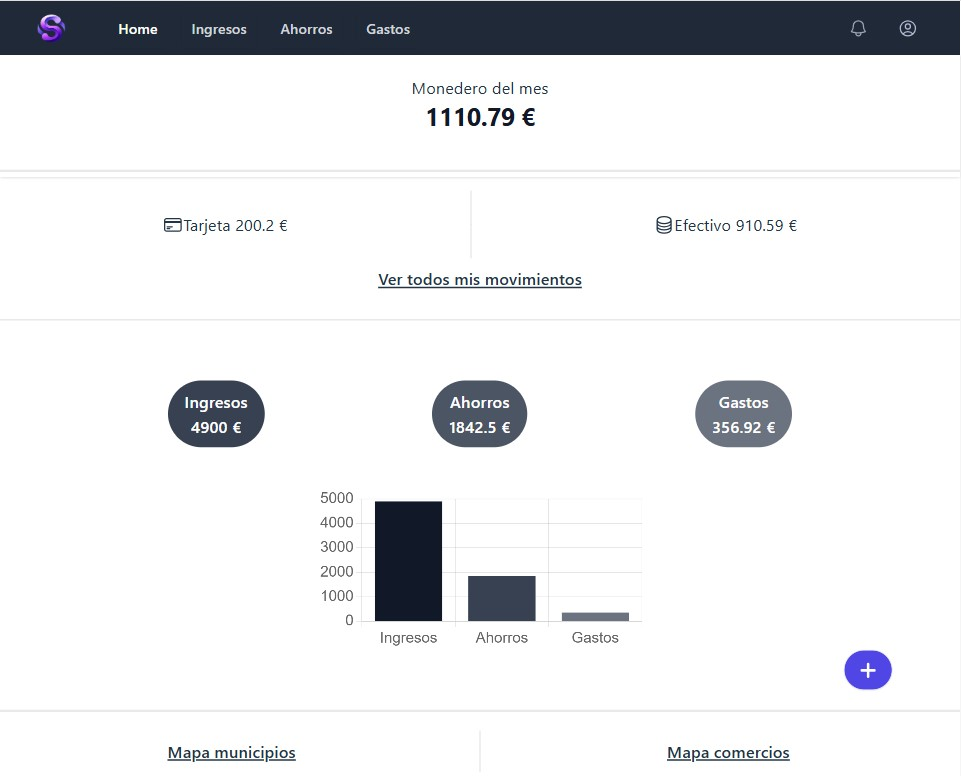
\includegraphics[width=\linewidth]{imagenes/M3-home.jpg}
    \caption{Gráfico de barras en la vista de inicio}
    \label{fig:bar_chart}
\end{figure}

\begin{figure}[ht!]
    \centering
    \begin{minipage}{0.45\textwidth}
        \centering
        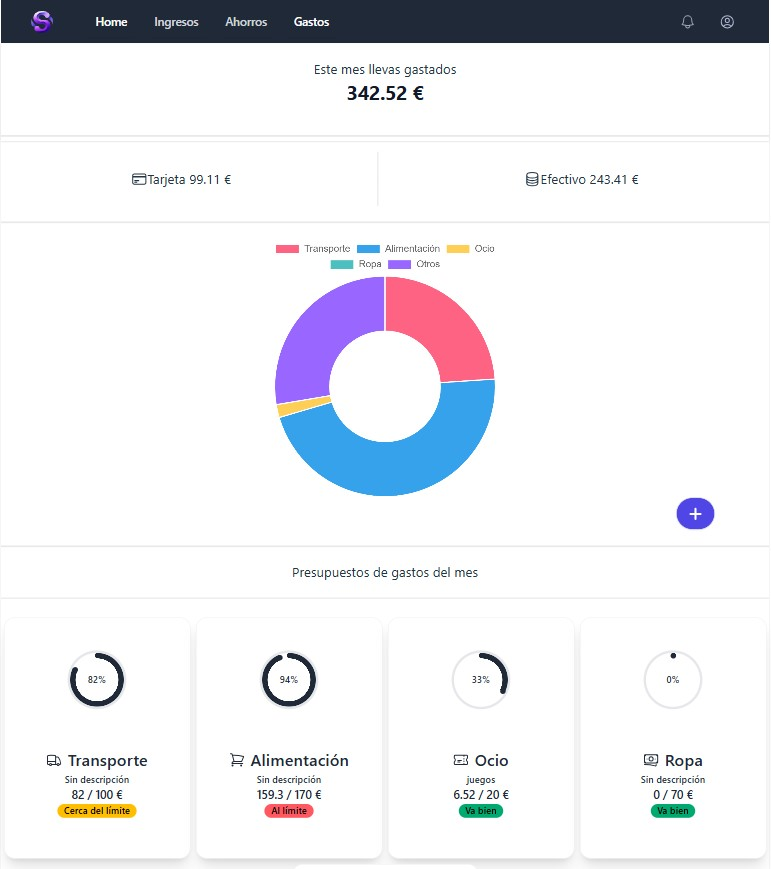
\includegraphics[width=\linewidth]{imagenes/M3-gastos.jpg}
    \end{minipage}\hfill
    \begin{minipage}{0.45\textwidth}
        \centering
        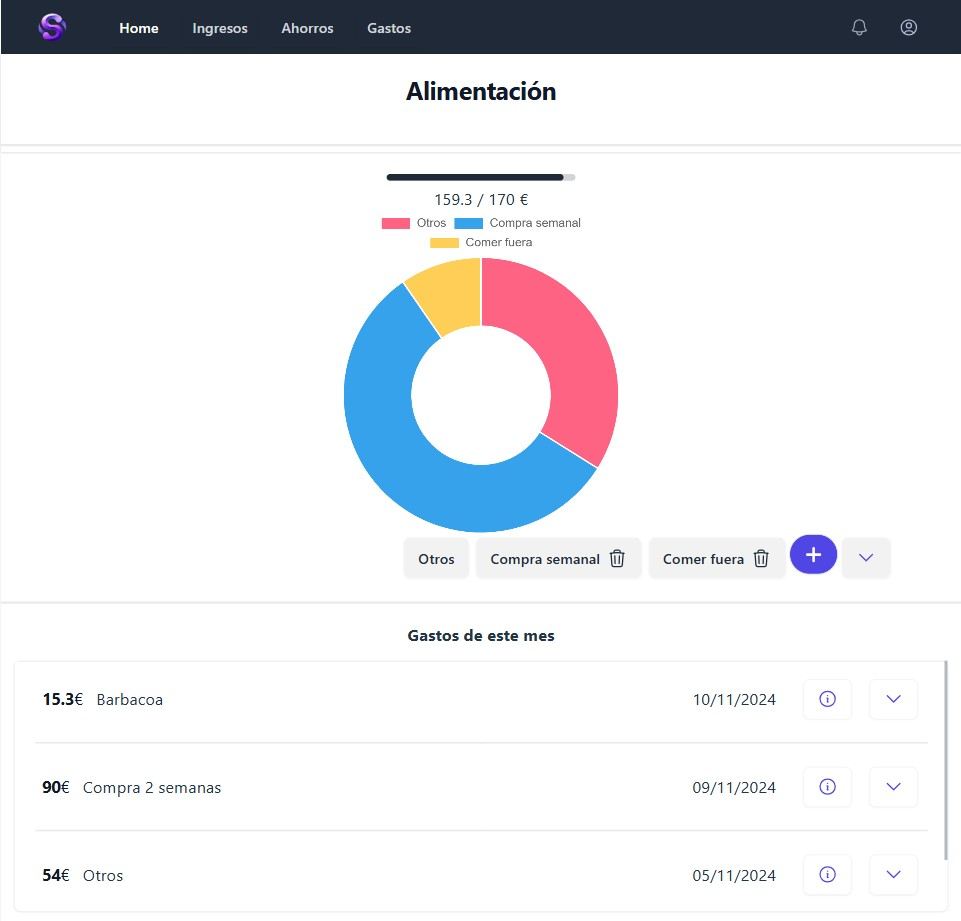
\includegraphics[width=\linewidth]{imagenes/M3-gastos-categoria.jpg}
    \end{minipage}
    \caption{Diagrama de anillo en la vista de gastos y la vista de categoría de gasto}
    \label{fig:doughnut_chart}
\end{figure}

\begin{figure}[ht!]
    \centering
    \begin{minipage}{0.45\textwidth}
        \centering
        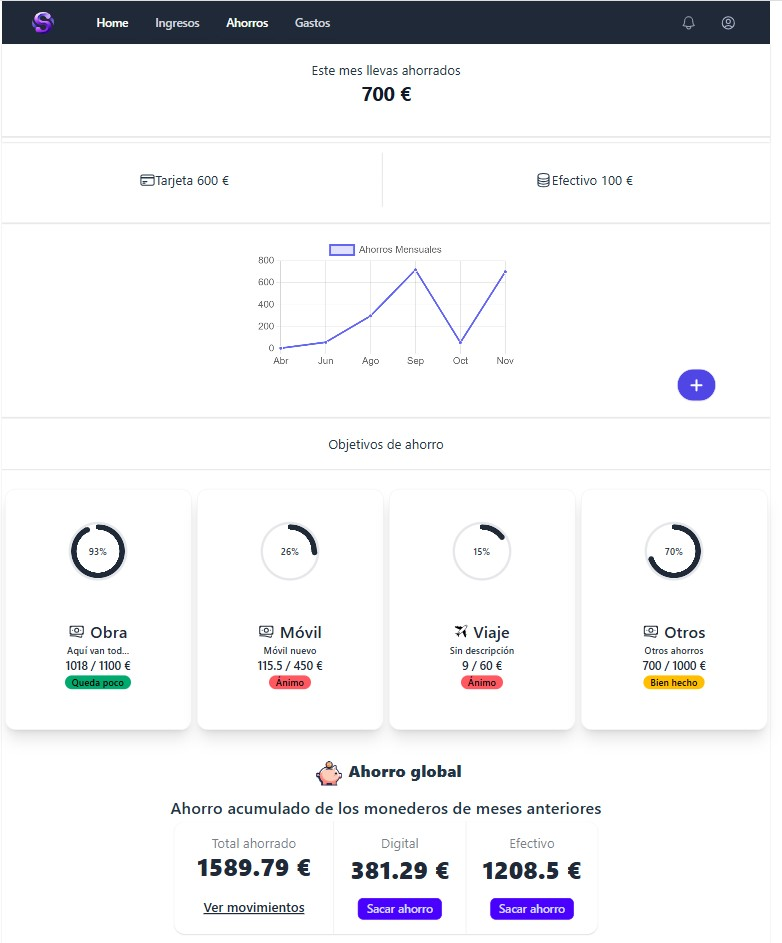
\includegraphics[height=70mm]{imagenes/M3-ahorros.jpg}
    \end{minipage}\hfill
    \begin{minipage}{0.45\textwidth}
        \centering
        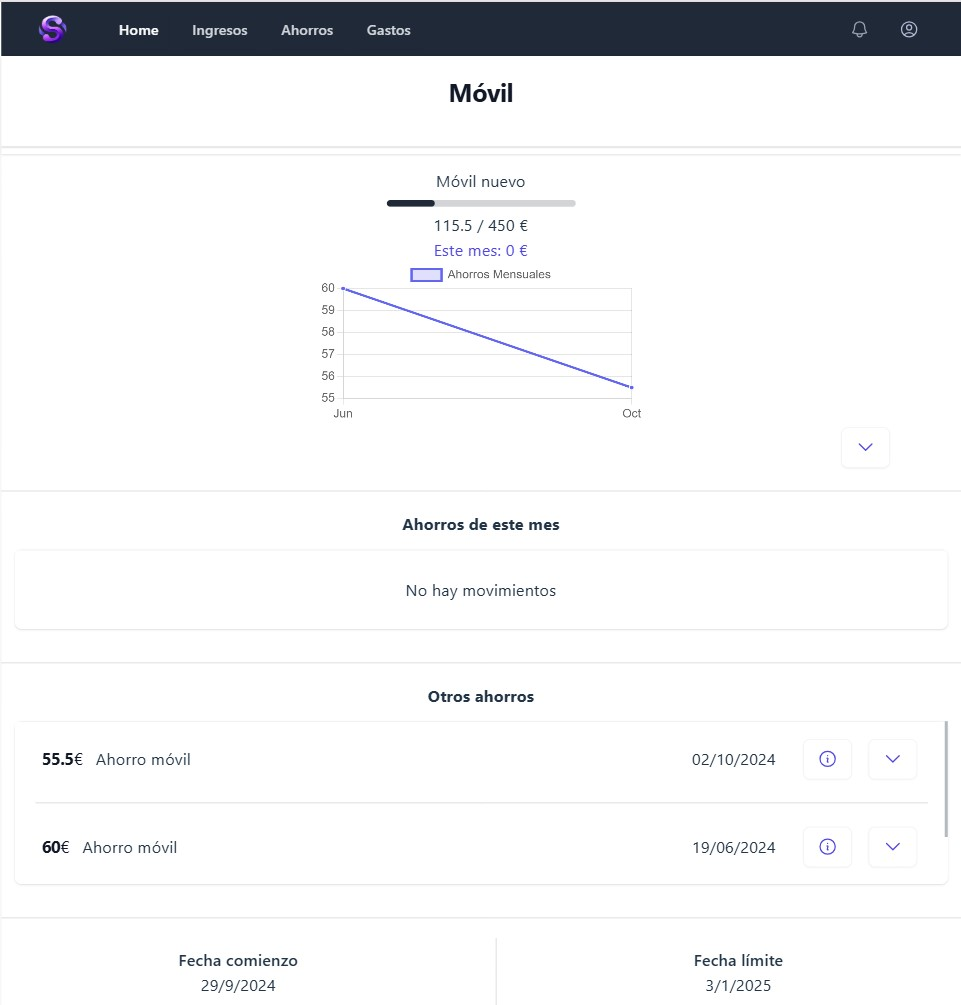
\includegraphics[height=70mm]{imagenes/M3-ahorros-objetivo.jpg}
    \end{minipage}
    \caption{Gráfico de líneas en la vista de ahorros y la vista de objetivo de ahorro}
    \label{fig:line_chart}
\end{figure}


\section{Relleno automático de gastos a partir de tickets (basado en OCR): Milestone 4}

La introducción manual de gastos en la aplicación puede resultar tediosa y lenta, especialmente cuando el usuario tiene que ingresar todos los detalles de un ticket de compra. No es sorprendente que, debido al esfuerzo involucrado, los usuarios dejen de completar los campos opcionales de las transacciones, lo que resulta en la pérdida de información valiosa para el análisis de sus gastos.

Dado este problema, se creó un objetivo al inicio del desarrollo de la aplicación, por el que se debía implementar un mecanismo para autorellenar los campos de un formulario en la aplicación a partir de la información obtenida de un ticket de compra. El usuario solo tendría que aportar una imagen del ticket y la aplicación se encargaría de extraer la información relevante y rellenar los campos correspondientes, posteriormente el usuario podría validar y modificar los datos si fuera necesario.

\subsection{Herramienta OCR}
La tecnología \textbf{OCR} (\textit{Reconocimiento óptico de caracteres}) permite la lectura de texto en imágenes, lo que facilita la extracción del texto en tickets de compra, sobre este texto se puede realizar un procesamiento posterior para obtener los datos necesarios. La implementación de esta tecnología en la aplicación permitirá al usuario ahorrar tiempo y esfuerzo en la introducción manual de gastos, mejorando la experiencia de usuario y aumentando la probabilidad de que complete todos los campos de las transacciones. Se evaluaron diferentes opciones para incorporar OCR.

\subsubsection{Criterios de búsqueda}
Debe ser compatible con Python. Para reducir costes del proyecto se busca una solución gratuita. 

\subsubsection{Criterios de selección}
\begin{itemize}
    \item Debe ser fácil de usar.
    \item Debe aportar una precisión aceptable en la lectura de texto.
    \item Su uso será frecuente y se espera agilidad, por lo que debe ser preferiblemente ligero y dar una respuesta rápida.
\end{itemize}

\subsubsection{Opciones compatibles con los criterios de búsqueda}
Eliminando las opciones de pago, no hay tantos OCRs gratuitos que ofrezcan una alta precisión. En general las herramientas o bien son menos precisas o tienen limitaciones de uso ofreciendo planes de pago para obtener una mayor precisión en la lectura de texto o disponibilidad de peticiones ilimitadas. Algunas de las opciones gratuitas son:
\begin{itemize}
    \item \textbf{Tesseract OCR}\\
        Es una herramienta de OCR de código abierto, que ha sido entrenada para reconocer una amplia variedad de fuentes y estilos de texto. La precisión del reconocimiento de texto puede variar, pero es suficiente para el propósito de la aplicación. Es ligera, rápida y no necesita de una configuración compleja.
    \item \textbf{EasyOCR}\\
        También es fácil de usar y ofrece una precisión similar a Tesseract. Necesita instalar PyTorch (biblioteca de aprendizaje automático, \textit{Machine Learning}) para su uso, lo que hace que sea más pesado.
    \item \textbf{Keras-OCR}\\
        Aunque puede ser potente en algunos casos, es necesario conocer Keras (biblioteca de aprendizaje profundo, \textit{Deep Learning}), lo que hace que la dificultad de uso sea mayor que en las anteriores y requiera de más configuración. 
\end{itemize}

\subsubsection{Opción seleccionada y justificación}
Se ha optado por la biblioteca \textbf{Tesseract OCR} con \textbf{pytesseract}, una interfaz para Tesseract fácil de usar, con buenos resultados y ampliamente usada para el procesamiento de imágenes. La precisión del reconocimiento de texto puede variar, pero es suficiente para el propósito de la aplicación.\\




El reconocimiento del texto de tickets por OCR presenta ciertas limitaciones cuando se emplean fuentes con estilos decorativos, letras cursivas, si la calidad de la imagen no es buena o si el ticket tiene partes que se han comenzado a borrar. Si bien se ha probado con el uso de APIs con versiones gratuitas para comparar la extracción (como \textit{Flashtext} o \textit{OCR.space}), el resultado de la lectura es muy similar al de Tesseract OCR, y se asume en este punto que la extracción de texto no será perfecta.

Dado el propósito de utilizar OCR en la aplicación, no será problema que la precisión no sea del 100\%, ya que el usuario podrá validar los datos si es necesario. Aún así, puesto que el objetivo para el que se usa OCR es procesar el texto obtenido para agilizar la introducción de datos en la aplicación, en el código desarrollado para tal uso, se ha incluido la implementación de numerosas funciones que validan los datos obtenidos. De esta forma (a excepción del campo con el nombre del comercio) \textbf{si no se puede asegurar el relleno correcto de un campo, no se autorellenará en el formulario para evitar un sobreesfuerzo al usuario}.


\subsection{Implementación de escaneo de tickets}
Al inicio se valoró usar alguna herramienta que permitiera extraer la información relevante de un ticket, sin embargo no se encontró ninguna herramienta gratuita y de acceso ilimitado que lo solucione. 

Se planteó la creación de un endpoint en el backend que reciba una imagen o PDF de un ticket de compra y devuelva el texto extraído de la imagen, ya procesado y listo para rellenar el formulario de creación de un nuevo gasto. Para ello, se ha creado un componente en React que permite al usuario subir una imagen y enviarla al backend para su procesamiento. Dada una entrada de imagen, la aplicación es capaz de devolver la información útil para rellenar los campos del formulario.

\begin{itemize}
    \item Solicitud POST. El cliente envía el archivo en una solicitud HTTP de tipo POST al endpoint.
    \item Guardado del archivo. El archivo se guarda temporalmente en el servidor.
    \item Procesamiento del archivo. Se comienza el procesamiento a partir de la ruta del archivo guardado.
    \item Procesamiento OCR. Uso de pytesseract para extraer texto del archivo.
    \item Extracción de información. Se procesa el texto extraído para obtener información específica del ticket como el nombre de la tienda, código postal, fecha, método de pago y monto total.
    \item Respuesta. La información extraída se devuelve como respuesta JSON al cliente.
\end{itemize}

Para el procesamiento de las imágenes se ha usado el módulo \textbf{Image} de la librería \textbf{Pillow}, una bifuración de PIL (\textit{Python Imaging Library}). Gracias a la simplicidad de pytesseract y PIL, el proceso de extracción de texto a partir de una imagen es sencillo, por lo que se decidió expandir la funcionalidad del script para que pueda procesar tanto imágenes como PDFs (puesto que actualmente algunos comercios envían el ticket de compra al usuario en este formato). Este cambio no supone inconvenientes en el desarrollo ya que la metodología de extracción de texto es la misma, solo es necesario añadir otra forma de cargar el archivo.

EL código para la extracción de los datos del ticket se ha realizado mediante un script en Python (de acuerdo al lenguaje de programación del backend). La implementación de la lectura de datos de un ticket a partir de una imagen o PDF sigue varios pasos, la funcionalidad del script se puede divididir en las tareas que se describen a continuación.


\subsubsection{Extracción del texto de la imagen}
El módulo \textbf{Image} de la biblioteca \textbf{PIL} \textit{Python Imaging Library}, permite cargar y manipular imágenes. Se realiza la carga de la imagen desde el archivo almacenado en el servidor y se extrae el texto completo del ticket con la función \textit{image\_to\_string} de \textbf{pytesseract}.
    
\begin{lstlisting}[language=Python, caption=Extracción de texto de una imagen]
    from PIL import Image
    import pytesseract

    def get_data_from_image_ticket(file_name):
        image = Image.open(f'app/tests/tickets_images/{file_name}')
        text = pytesseract.image_to_string(image)

        return get_data(text)
\end{lstlisting}

\subsubsection{Extracción del texto del PDF}
Inicialmente la extracción se hizo con la biblioteca \textbf{PyMuPDF} por su fama de ser muy rápida en la lectura de PDFs. Con un par de ejemplos se encontraron problemas en la lectura de los archivos que contenían datos estructurados en columnas, algo usual en los tickets, ya que presentan tablas con los productos comprados. Por ello finalmente se optó por \textbf{PDF Plumber}, una biblioteca de Python que permite extraer directamente texto e información de los PDFs. De la misma forma que con las imágenes, se carga el archivo y se extrae el texto completo del ticket. Se usará esta función en lugar de la anterior cuando la extensión del archivo sea PDF.

\begin{lstlisting} [language=Python, caption=Extracción de texto de un PDF]
    import pdfplumber

    def get_data_from_pdf_ticket(file_name):
        text = ""
        with pdfplumber.open(f'app/tests/tickets_PDFs/{file_name}') as pdf:
            for page in pdf.pages:
                page_text = page.extract_text()
                if page_text:
                    text += page_text + '\n'
        
        return get_data(text)
\end{lstlisting}

\subsubsection{Análisis de los elementos en un ticket}
Una vez obtenida la cadena de texto, ya sea desde la imagen o el PDF, se inició el proceso de identificación de los componentes en un ticket. Este proceso comienza con un análisis exhaustivo de diversos tickets por parte del desarrollador para determinar la información relevante que se puede extraer porque se presenta de forma general en ellos: nombre del comercio, dirección, código postal, nombre del municipio, NIF, fecha, método de pago e importe total (Figura \ref{fig:componentes_ticket}).

De ellos, se valoró cuáles serían de utilidad para completar el formulario de creación de una transacción de gasto (se puede ver la vista del formulario en la Figura \ref{fig:formulario_gasto}) e implementar el mecanismo para extraerlos.

\begin{figure}[ht!]
    \centering
    \begin{minipage}{0.45\textwidth}
        \centering
        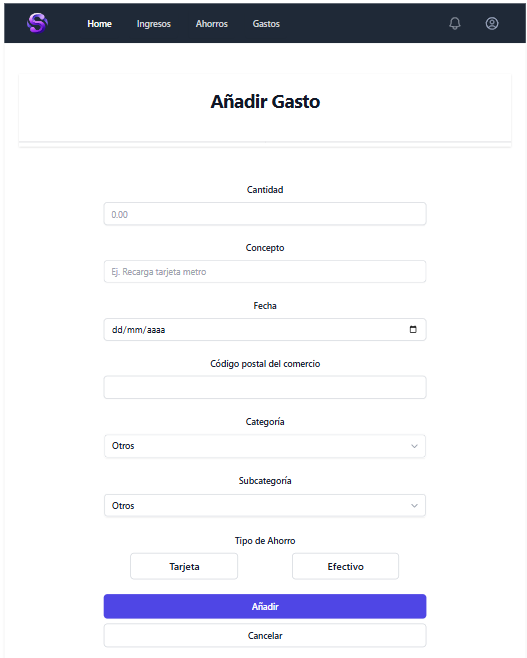
\includegraphics[height = 70mm]{imagenes/formulario_gasto.png}
        \caption{Formulario de creación de un gasto}
        \label{fig:formulario_gasto}
    \end{minipage}\hfill
    \begin{minipage}{0.45\textwidth}
        \centering
        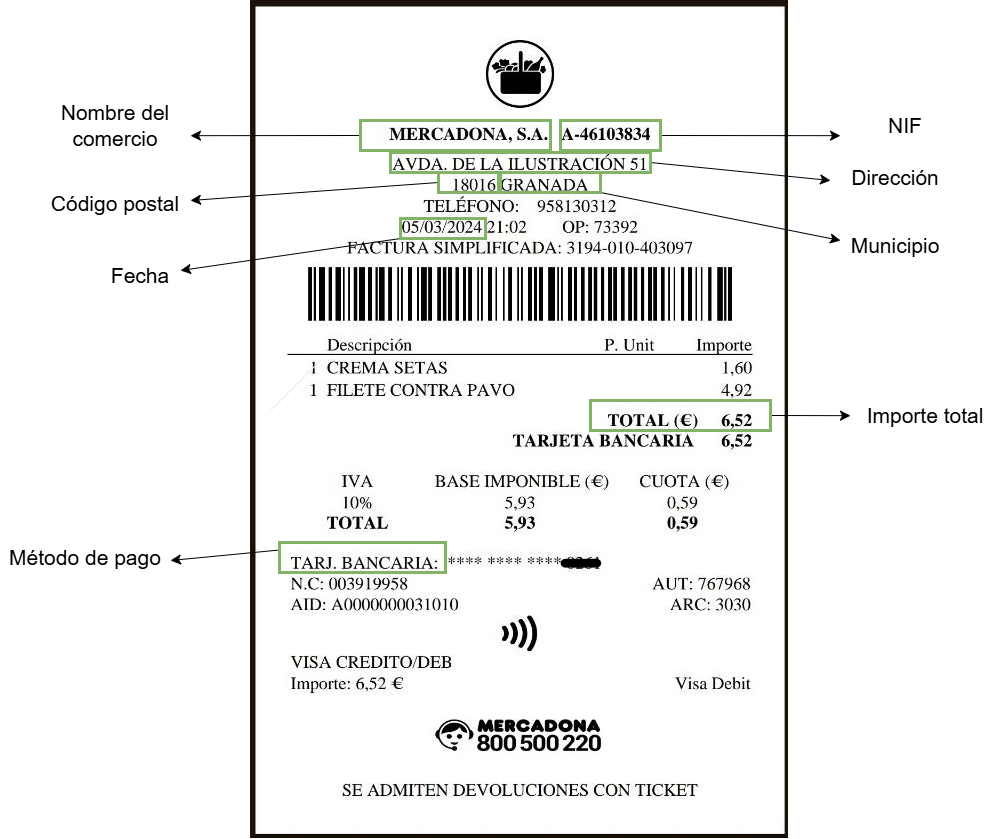
\includegraphics[height = 70mm]{imagenes/componentes_ticket.png}
        \caption{Componentes de un ticket}
        \label{fig:componentes_ticket}
    \end{minipage}
\end{figure}

\subsubsection{Extracción de campos}
Dado que los tickets suelen ser textos breves, en la mayoría de casos se optó por el uso de expresiones regulares (regex) para buscar y extraer información específica. Las expresiones regulares son especialmente útiles para esta tarea, ya que permiten definir patrones precisos de búsqueda y son rápidas en volúmenes reducidos de texto. Así, se crean funciones específicas para identificar y extraer cada dato relacionado a un campo del formulario.

Cada función es llamada desde una función principal que recibe el texto extraído del ticket y devuelve un diccionario con los campos identificados y el valor extraído. En caso de no encontrar un campo, se devuelve en él valor 'desconocido'.

\begin{lstlisting} [language=Python, caption=Extracción los campos del ticket]
    # returns a dictionary with ticket data
    def get_data(text):
        text = text.lower()

        payment_method = get_payment_method(text)
        date = get_date(text)
        shop_data = get_shop_data(text)
        total_amount = get_total_amount(text)

        ticket_data = {
            'shop_name': shop_data['shop_name'],
            'shop_postal_code': shop_data['postal_code'],
            'date': date,
            'payment_method': payment_method,
            'total_amount': total_amount,
        }

        return ticket_data
\end{lstlisting}


\begin{itemize}
    \item \textbf{Método de pago.} Se determina si el método de pago es en efectivo o tarjeta, o si es desconocido. Primero busca palabras clave directas que identifiquen un método u otro como que aparezca la cadena 'efectivo'. Si no las encuentra cuenta las ocurrencias de palabras clave relacionadas para hacer una determinación basada en la frecuencia de estas palabras.
    
    \begin{lstlisting}[language=Python, caption=Extracción del método de pago en un ticket]
    # returns 'tarjeta', 'efectivo' or 'desconocido' if not found
    def get_payment_method(text):
        payment_method = 'desconocido'
    
        if 'tarjeta' in text:
            payment_method = 'tarjeta'
        elif 'efectivo' in text or 'contado' in text:
            payment_method = 'efectivo'
        else:
            count_tarjeta = 0
            count_efectivo = 0
    
            keywords_tarjeta = ['visa', 'mastercard', 'debito', 'debit', 'credito', 'credit', 'contactless', 'nfc', 'cuenta','caixabank', 'bbva', 'trj', 'jeta', 'tarj', 'tanjeta']
            keywords_efectivo = ['cambio', 'entrega', 'entregado', 'efect', 'entr', 'cont']
    
            count_tarjeta = sum(text.count(keyword) for keyword in keywords_tarjeta)
            count_efectivo = sum(text.count(keyword) for keyword in keywords_efectivo)
    
            if count_tarjeta >= 2 and count_tarjeta > count_efectivo:
                payment_method = 'tarjeta'
            elif count_efectivo >= 2 and count_efectivo > count_tarjeta:
                payment_method = 'efectivo'
                
        return payment_method
    \end{lstlisting}

    \item \textbf{Fecha.} Se busca la fecha, que puede aparecer en diferentes formatos, se han contemplado varios formatos posibles (\textit{dd\_mm\_yyyy, dd\_mm\_yy, yyyy\_mm\_dd}). Primero elimina los espacios en blanco del texto y luego intenta extraer la fecha en cada uno de los formatos mencionados, estableciendo prioridad en los intentos ya que el formato de fecha más frecuente en España es \textit{dd\_mm\_yyyy}. Si no se encuentra una fecha en ninguno de los formatos, devuelve 'desconocido'. Para cada formato se comprueba la validez de la fecha, y que no se extraiga más de una fecha en el texto (ya que en algunos tickets se muestra la fecha límite para devoluciones), si no se cumple alguna de estas condiciones se devuelve 'desconocido'.

    \begin{lstlisting} [language=Python, caption=Extracción la fecha en un ticket]
    # returns date with dd/mm/aaaa format o 'desconocido' if not found
    def get_date(text):
        date = 'desconocido'
        text = text.replace(' ', '')

        date = get_date_dd_mm_yyyy(text)
        if date == 'desconocido':
            date = get_date_dd_mm_yy(text)   
            if date == 'desconocido':
                date = get_date_yyyy_mm_dd(text)

        return date
    \end{lstlisting}

    \item \textbf{Datos del comercio.} Se extrae información relevante sobre una tienda, específicamente el nombre de la tienda y el código postal. Utiliza funciones auxiliares (\textit{get\_postal\_code, get\_street, get\_shop\_name}) para obtener estos datos y los organiza en un diccionario que luego devuelve.
    
    Para las extracciones de los campos concretos se han usado expresiones regulares.  

    \begin{lstlisting} [language=Python, caption=Extracción de los datos del comercio]
    # returns a dictionary with shop data
    def get_shop_data(text):
        postal_code = get_postal_code(text)
        street = get_street(text, postal_code)
        shop_name = get_shop_name(text)

        shop_data = {
            'shop_name': shop_name,
            'postal_code': postal_code,
        }
        return shop_data
    \end{lstlisting}

\subitem \textbf{Código postal}. Se busca un patrón de cinco dígitos aislado en el texto, se asume que en la mayoría casos este será el código postal de la tienda. Si no se encuentra, devuelve 'desconocido'. \label{codigo_postal}
    \begin{lstlisting} [language=Python, caption=Extracción del código postal]
    # returns postal code or 'desconocido' if not found
    def get_postal_code(text):
        postal_code = 'desconocido'

        match = re.search(r'\n[\s\n]*\d{5}[\s\n.-]', text)
        if match:
            match_postal_code = re.search(r'\d{5}', match.group(0))
            postal_code = match_postal_code.group(0)

        return postal_code
    \end{lstlisting}


\subitem La función para el \textbf{nombre de la tienda} toma un texto y una calle como entrada y trata de extraerlo: busca patrones específicos que coincidan con nombres de tiendas que terminan en \textit{S.A.} o \textit{S.L.} y si esa búsqueda no encuentra coincidencias, toma las primeras dos líneas del texto. Si encuentra una coincidencia elimina la calle (dirección) si se ha añadido erróneamente dentro del nombre. Finalmente, devuelve el nombre de la tienda o 'desconocido' si no se encontró ninguna coincidencia.
    \begin{lstlisting} [language=Python, caption=Extracción del nombre de la tienda, literate={á}{{\'a}}1 {é}{{\'e}}1 {í}{{\'i}}1 {ó}{{\'o}}1 {ú}{{\'u}}1 {ñ}{{\~n}}1 {Á}{{\'A}}1 {É}{{\'E}}1 {Í}{{\'I}}1 {Ó}{{\'O}}1 {Ú}{{\'U}}1 {Ñ}{{\~N}}1]
    # returns shop name or 'desconocido' if not found
    def get_shop_name(text, street):
        shop_name = 'desconocido'

        text = re.sub(r'\r;)(', ' ', text)

        match = re.search(r'[a-zá-ú]+.*[sS]\.[aAlL]+', text) # S.A. (Sociedad Anónima) // S.L. (Sociedad Limitada)

        if not match:
            match = re.search(r'[a-zá-ú].+\n.*\n', text) # first two lines
        if match:
            shop_name = match.group(0).replace('\n', ' ').replace('\r', ' ')
            if street in shop_name:
                shop_name = shop_name.replace(f'{street}', '')

        return shop_name
    \end{lstlisting}

En esta extracción se presenta la dificultad de que los nombres de tiendas no suelen seguir un patrón claro, en el texto del ticket es fácil perder la referencia de qué es el nombre de la tienda, qué es la dirección o la descripción de un artículo. Por ello se decidió extraer el nombre por su posición al inicio del texto si no se encuentra un patrón que lo identifique. Además, como alternativa al uso de patrones se probaron bibliotecas de procesamiento de lenguaje natural como spaCy para extraer entidades (como nombres de tiendas o ciudades) usando un modelo preentrenado en español. Se intentó también
la extracción con Flashtext para buscar coincidencias de nombres de tiendas en una lista de
comercios conocidos. La extracción del NIF se resolvió con patrones específicos,
y aunque se consideró relacionarlo con el nombre del comercio a través de APIs,
su uso se descartó para este proyecto debido a las restricciones en el volumen de
consultas que ofrecen los planes gratuitos

    \item \textbf{Importe total.} Este procesamiento es el más complejo, ya que se buscan cadenas coincidentes con el formato esperado, y en este caso, todos los números del ticket tienen el mismo formato. Esto puede generar ambigüedad en la extracción del importe total.

    El aspecto clave para conseguir la cantidad total reside precisamente en esta palabra de la que va acompañada: 'total'. Se busca la palabra 'total' en el texto seguida de un número con decimales y posiblemente una representación de la divisa: el símbolo \textit{€}, la palabra \textit{euro} o simplemente la letra \textit{e}.  Si no se encuentra se realizan búsquedas alternativas, con la palabra 'importe', 'venta' o partes de ellas. Las coincidencias obtenidas se almacenan en una lista de Python que se irá depurando, eliminando de ella los precios que indican un total de IVA, un total de descuento, o si se encuentra un número al final de línea (cuando no hay descuentos) mayor que los de la lista de candidatos. De modo que en casos como el de la Figura \ref{fig:get_total_amount_peculiaridades} se extraería el importe total de 29,96 porque se descartaría 24,00 de la lista de candidatos.

    \begin{figure}[ht!]
        \centering
        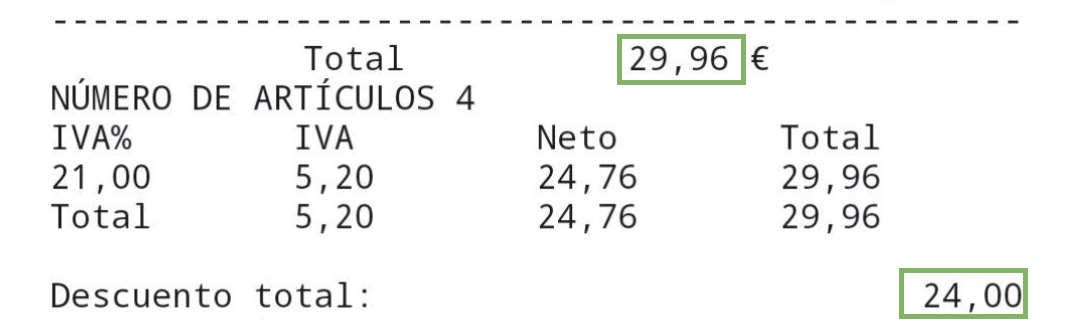
\includegraphics[height=30mm]{imagenes/get_total_amount_peculiaridades.png}
        \caption{Ticket con descuento}
        \label{fig:get_total_amount_peculiaridades}
    \end{figure}

Texto leído del fragmento de la Figura \ref{fig:get_total_amount_peculiaridades}
    \begin{lstlisting}[literate={€}{{\euro}}1 {á}{{\'a}}1 {é}{{\'e}}1 {í}{{\'i}}1 {ó}{{\'o}}1 {ú}{{\'u}}1 {ñ}{{\~n}}1]
        \n\n \n\n \n\n \n\ntotal 29,96 €\nnumero de articulos 4\niva% iva neto total\n21,00 5,20 24,76 29,96\ntotal 5,20 24,76 29,96\ndescuento total: 24,00
    \end{lstlisting}

    \begin{lstlisting} [language=Python, caption=Extracción del importe total]
    # returns total amount or 'desconocido' if not found
    def get_total_amount(text):
        total_found = False
        total_amount ='desconocido'
        total_from_eol_prices = 0
        total_from_candidates = 0
        percentage_prices = get_iva_prices(text)
        discount_prices = get_discount_prices(text)

        invalid_prices = percentage_prices + discount_prices

        if not discount_prices:
            eol_prices = get_eol_prices(text, invalid_prices)         
            if eol_prices:
                total_from_eol_prices = max(eol_prices)
        
        total_prices = get_total_prices(text, invalid_prices)

        if total_prices:
            total_found = True
            total_from_candidates = max(total_prices)      
        
        if total_found:
            if total_from_candidates >= total_from_eol_prices:
                total_amount = str(total_from_candidates)

        return total_amount
    \end{lstlisting}
\end{itemize}


\subsubsection{Problemas encontrados}
La identificación de cadenas de texto sin patrones claros como el nombre de la tienda comprometen la precisión de los resultados. La dificultad se agrava debido a que los tickets contienen caracteres especiales, saltos de línea y símbolos que, al mezclarse en el texto, dificultan identificar palabras o frases completas, así como ciertas tipografías que usan los nombres de comercios. 

El resto de los campos del formulario están sometidos a validaciones estrictas para asegurar la calidad de los datos; si no cumplen con los requisitos, el sistema no registra los valores. Este enfoque prioriza la precisión, de modo que el usuario evite corregir manualmente campos incorrectos. A diferencia del resto, para simplificar el proceso de entrada de datos, el campo 'concepto' de gasto se rellena con el nombre del comercio aunque no sea una coincidencia perfecta, ya que solo sirve como referencia identificativa de la transacción.

El resto de información que se ha procesado pero no ha sido relevante o no ha sido posible extraerla con precisión, se ha descartado. Por ejemplo, la dirección del comercio (calle y municipio), el NIF, el IVA o si había descuentos. Los métodos implementados están disponible en el repositorio donde se aloja el proyecto, aunque se ha decidido no incluirlos en la aplicación para no sobrecargar al usuario con información innecesaria, manteniendo así la simplicidad de la interfaz.


\subsubsection{Pruebas}
Se guardaron 24 tickets de diferentes comercios en formato de texto (usando las funciones de extracción de texto implementadas) para realizar pruebas con el script de extracción de datos. Estos tickets sirven como base para realizar pruebas controladas que permitan medir la capacidad del script para identificar correctamente los campos relevantes. Para una representación más realista, se incluyeron tickets en formato tanto de imagen como PDF, procurando que las muestras tuvieran variedad de fuentes y estilos de texto, así como tickets con errores de impresión o deterioro.

Se empleó \textbf{pytest} para desarrollar pruebas unitarias para cada una de las funciones encargadas de extraer los campos específicos del ticket, como el nombre del comercio, el importe total, la fecha y otros datos de interés. Cada función se probó con múltiples casos representativos, verificando que los valores devueltos fueran los esperados. Esto permitió observar cómo respondía el código desarrollado ante diferentes formatos y disposición de elementos en los tickets. A través de estas pruebas, la implementación se ajustó progresivamente para maximizar la precisión en la extracción de datos.

\begin{lstlisting} [language=Python, caption=Tests de extracción de fechas]
    # returns total amount or 'desconocido' if not found
    def test_get_date_dd_mm_yy():
        expected = ["desconocido", "12/06/2024", "desconocido", "desconocido", "desconocido", "16/08/2024",
                    "15/06/2024", "24/06/2024"]
        tickets_dd_mm_yy = [text[4], text[6], text[7], text[10], text[18], text[19],
                            text[21], text[22]]
        i = 0
        for ticket in tickets_dd_mm_yy:
            with open(f'{base_path}{ticket}', 'r') as file:
                ticket_str = file.read().lower()
                assert get_date(f'{base_path}{ticket_str}') == expected[i]
                i += 1

    def test_get_date_yyyy_mm_dd():
        # on ticket: 3(2024-04-23)
        expected = ["23/04/2024", "desconocido"]
        tickets_yyyy_mm_dd = [text[3]]
        i = 0
        for ticket in tickets_yyyy_mm_dd:
            with open(f'{base_path}{ticket}', 'r') as file:
                ticket_str = file.read().lower()
                assert get_date(f'{base_path}{ticket_str}') == expected[i]
                i += 1

    def test_get_date_mix():
        # on: (09/05/21) -> solo fechas de 2024 en adelante
        expected = ["01/01/2024", "02/02/2024", "03/03/2024", 
                    "04/04/2024", "05/05/2024", "06/06/2024", 
                    "07/07/2024", "08/08/2024", "09/09/2024","desconocido"]
        dates_mix = ["srd01/01/2024", "rtnjs 02-02-2024", "rtrju 03.03.2024", 
                    "03948n 04/04/24", "asff05-05-24", "06.06.24dvgsd", 
                    "2024-07-07", "2024/08/08 sdr", "2024.09.09 999", "09/05/21"]
        i = 0
        for date in dates_mix:
            assert get_date(date) == expected[i]
            i += 1
\end{lstlisting}

\subsubsection{Conclusiones}
El uso de OCR para la extracción de datos de tickets ha sido un reto interesante y ha permitido mejorar la experiencia del usuario en la aplicación. Aunque la precisión de la extracción no es del 100\%, el script desarrollado ha demostrado ser capaz de extraer información relevante de los tickets de compra, lo que facilita la introducción de gastos en la aplicación. En cuanto a la implementación, se ha logrado un buen equilibrio entre la precisión y la velocidad de procesamiento, lo que permite al usuario ahorrar tiempo y esfuerzo en la introducción manual de gastos y aumenta la probabilidad de que los usuarios completen todos los campos de las transacciones.

En la Tabla \ref{tab:pruebas_extraccion_datos} se muestra un resumen de algunos resultados obtenidos en las pruebas realizadas con el script de extracción de datos de tickets. Se puede observar que la precisión de la extracción varía según el campo y el formato del ticket, pero en general, el script ha demostrado ser capaz de identificar correctamente los campos relevantes en la mayoría de los casos.

\begin{landscape}
    \begin{table}[]
    \begin{tabular}{|l|l|l|l|l|l|l|l|}
    \hline
    \textbf{Nombre del Ticket} & \textbf{Nombre Comercio (concepto)} & \textbf{Código Postal} & \textbf{Total} & \textbf{Fecha} & \textbf{Método de Pago} & \textbf{Observaciones sobre el Ticket} & \textbf{Errores en la Extracción de Campos} \\ \hline
    01\_ikea & Tkea ibfrica, s.a & 18100 & 2.99 & 05/08/2024 & Tarjeta & Formato de fecha en el ticket: 05.08.24 & Lectura del nombre casi perfecta, error en dos caracteres. \\ \hline
    02\_ikea\_captura\_pantalla & Ikea iberica, s.a. & 18100 & 103.0 & 26/03/2024 & Tarjeta &  &  \\ \hline
    03\_casa\_del\_libro & Liente & desconocido & 9.85 & 23/04/2024 & Tarjeta & Formato de fecha en el ticket: 2024-04-23 & Error en la lectura del nombre; no lee el código postal. \\ \hline
    04\_lefties & Lefties & desconocido & 17.99 & 01/02/2024 & Tarjeta & No incluye código postal &  \\ \hline
    05\_primor & Megapr i mor, s.l & 18100 & 4.3 & 12/06/2024 & Tarjeta & Formato de fecha en el ticket: 12/06/24 &  \\ \hline
    06\_mercadona & Mercadona, s.a & 18016 & desconocido & 17/06/2024 & Tarjeta &  &  \\ \hline
    07\_mercadona\_captura\_pantalla & Mercadona, s.a & 18016 & 6.52 & 05/03/2024 & Tarjeta &  & No lee el código postal. \\ \hline
    08\_ecu & Cerveceria ecu §2.521.648k & 18008 & 22.3 & 23/06/2024 & Efectivo &  & Error parcial en la lectura del nombre. \\ \hline
    09\_hym\_captura\_pantalla & Comprarent... q sl © & 18100 & 2.99 & 24/06/2024 & Tarjeta & Incluye precio de descuento mayor al total & Error en la lectura del nombre. \\ \hline
    11\_margaritas\_blancas & Margaritas blancas & desconocido & 6.5 & 27/04/2024 & Efectivo & No incluye código postal &  \\ \hline
    12\_carrefour\_pdf & Centros comerciales carrefour s.a & desconocido & 49.78 & 19/08/2024 & Tarjeta & PDF. No tiene código postal por ser compra online &  \\ \hline
    13\_mercadona\_pdf & Mercadona, s.a & 18016 & 3.5 & 09/04/2024 & Tarjeta & PDF recibo de compra física &  \\ \hline
    \end{tabular}
    \caption{Pruebas de extracción de datos en tickets de diferentes comercios.}
    \label{tab:pruebas_extraccion_datos}
    \end{table}
    \end{landscape}
    


\section{Incorporación de mapas y tiendas: Milestone 5}
Cuando los usuarios añaden gastos en la aplicación el único componente que identifica a la tienda es el nombre de la misma (que suele indicarse en el concepto) de la transacción. Sin embargo, se considera que sería útil para los usuarios poder visualizar en un mapa la ubicación de las tiendas donde han realizado sus compras. Esto les permitiría tener una visión más clara de sus gastos que permite identificar patrones de consumo y comparar precios entre diferentes tiendas. Por otro lado, aprovechando que en la lectura de tickets se extrae el código postal de la tienda, se representan los gastos en un mapa de España agrupados por municipios, lo que permitiría a los usuarios analizar su gasto por zonas geográficas.\\

Partiendo de las premisas anteriores, se pueden diferenciar varios aspectos a tratar para implementar esta funcionalidad:

\begin{itemize}
    \item Integrar mapas interactivos en la aplicación. Conlleva la integración de una herramienta que permita la representación de mapas y la localización de elementos en ellos, que independientemente de cómo se agrupen (por localidad o por comercio), se representarán como puntos en el mapa con cierta información relacionada.
    \item  Para los gastos por municipios, se debe abordar la obtención de coordenadas geográficas a partir de un código postal, que permitirá representar los gastos por municipios.
    \item Derivado del apartado anterior, se debe abordar la obtención de comercios y sus coordenadas geográficas, de forma que se puedan representar las tiendas en un mapa.  
\end{itemize}


\subsection{Herramienta para representación de mapas}
\subsubsection{Criterios de búsqueda}
Debe ser compatible con React y permitir el uso de datos de OpenStreetMap para visualizar mapas en la aplicación. \textbf{OpenStreetMap} es una base de datos de mapas de código abierto que ofrece datos geográficos detallados y actualizados de todo el mundo. Es una alternativa a los servicios de mapas comerciales como Google Maps y ofrece una API gratuita y de código abierto que permite a los desarrolladores acceder a sus datos y utilizarlos en sus aplicaciones\cite{openstreetmap_about}.

\subsubsection{Criterios de selección}
\begin{itemize}
    \item Debe disponer de una amplia documentación.
    \item Debe ser ligera (o no muy pesada).
    \item Debe ofrecer una integración sencilla con React.
\end{itemize}

\subsubsection{Opciones compatibles con los criterios de búsqueda}
\begin{itemize}
    \item \textbf{Leaflet}\\
        Esta biblioteca ofrece un equilibrio muy bueno entre funcionalidad y simplicidad. Es ligera y fácil de usar, con una documentación extensa y una amplia comunidad de usuarios. Leaflet tiene wrappers para React que facilitan su integración en aplicaciones React y ofrece una amplia variedad de plugins y extensiones para personalizar los mapas.
    \item \textbf{OpenLayers}\\
        Es una biblioteca más compleja y pesada que Leaflet, pero ofrece una mayor cantidad de funcionalidades y opciones de personalización. Documentación suficiente aunque algo más técnica. OpenLayers es una buena opción para aplicaciones que requieren un alto grado de personalización y funcionalidades avanzadas.
    \item \textbf{Pigeon Maps}\\
        Es una biblioteca ligera y fácil de usar que está diseñada específicamente para React. Aunque no es tan popular como Leaflet, lo que puede limitar la disponibilidad de plugins y extensiones y menor documentación.
\end{itemize}

\subsubsection{Opción seleccionada y justificación}
Se ha optado por la biblioteca \textbf{Leaflet} por su equilibrio entre funcionalidad y simplicidad, y su integración sencilla con React. Leaflet ofrece el wrapper \textit{react-leaflet} para facilitar la integración de mapas interactivos en aplicaciones React, conviertiendo el mapa en un componente de React que puede personalizarse fácilmente y reutilizarse en la aplicación.


\subsection{Herramienta para la obtención de las coordenadas geográficas de una localidad}
A la hora de representar los gastos por localidad, se necesita una herramienta que permita obtener las coordenadas geográficas de una localidad a partir de su código postal (siendo el código el único dato geográfico recogido hasta ahora en el formulario de un gasto). 

Se debe desarrollar en el backend de la aplicación una función que, dado un código postal, devuelva las coordenadas geográficas de la localidad asociada a ese código postal. Para ello, se necesita una herramienta que permita realizar esta conversión de forma sencilla y eficiente.\\

A la hora de agrupar todas las transacciones del usuario por localidades, se debe tener en cuenta que para un mismo lugar pueden existir varios códigos postales\footnote{Los códigos postales se asignan principalmente a localidades, pero existen otras asignaciones: las capitales de provincia y algunas grandes ciudades suelen estar divididas en varias zonas postales, mientras que hay lugares donde un mismo código se aplica a varias localidades cercanas\cite{cp-wikipedia}.}, lo que puede provocar inconsistencias en la representación de datos.

\subsubsection{Criterios de búsqueda}
\begin{itemize}
    \item Debe proporcionar las coordenadas y el nombre de la localidad asociados a un código postal.
    \item Debe permitir consultas gratuitas.
    \item Debe ser compatible con Python.
    \item Debe ser sencilla de integrar en la aplicación.
\end{itemize}
\subsubsection{Criterios de selección}
\begin{itemize}
    \item Preferencia por APIs con límites de consulta elevados o de acceso completo gratuito. Puesto que el número de consultas es proporcional a la cantidad de transacciones, se debe tener en cuenta el límite de consultas que permita la herramienta.
    \item Se valorará positivamente una respuesta rápida a las consultas.
\end{itemize}

\subsubsection{Opciones compatibles con los criterios de búsqueda}
\begin{itemize}
    \item \textbf{OpenStreetMap Nominatim API}\\
    Es un servicio de geocodificación basado en OpenStreetMap. Es una API gratuita, pero está sujeta a limitaciones en el número de consultas por segundo que se pueden realizar, lo que dependiendo del número de usuarios de la aplicación, puede ser un problema.
    \item \textbf{pgeocode} (Python Geocode)\\
    Es una biblioteca de Python, por lo que trabaja con datos descargados en el sistema y no tiene límite de consultas. Es una herramienta sencilla de usar y ofrece una integración directa con Python.
\end{itemize}

\subsubsection{Opción seleccionada y justificación}\label{sec:justificacion_pgeocode}
Python Geocode, por sus prestaciones, es la mejor opción para obtener las coordenadas de un punto de referencia de la localidad asociada a dicho código postal, permitiendo así la representación geográfica del gasto. Sin embargo, ninguna de las herramientas solucionan de forma directa el problema de los códigos postales, ya que no se puede garantizar que el punto de referencia obtenido sea único para representar todos los gastos en la localidad, y realizar comprobaciones adicionales (sumado al tiempo de respuesta de las consultas) puede compromenter la eficiencia.\\
Teniendo en cuenta lo anterior, se decide que la mejor solución será crear una tabla en la base de datos (ya que el tamaño de los datos a almacenar no es demasiado grande) que asocie cada código postal con las coordenadas geográficas de un único punto de referencia de la localidad. Aprovechando la personalización de la tabla para garantizar la unicidad de los códigos postales, las ventajas de usar base de datos que optimizan las consultas y en especial debido a que los códigos postales son datos estáticos que no cambian con frecuencia.\\
De esta forma, se garantiza que la consulta de los gastos por localidades sea precisa y eficiente.


\subsection{Herramienta para obtención de las coordenadas geográficas de un comercio}
Se necesita una herramienta que facilite la identificación de un comercio para que el usuario lo pueda añadir en el formulario de creación de un gasto, de forma que se pueda representar en el mapa la ubicación de la tienda.

Teniendo en cuenta que no se quiere complicar al usuario con la introducción de datos, no se le solicitará la dirección completa del lugar, se pretende localizar un comercio en un mapa a partir de su nombre y código postal, puesto que son los únicos datos para identificarlo recogidos en el formulario.

Una vez que el usuario identifique el comercio, se deben obtener las coordenadas geográficas de la tienda para poder representarla en el mapa.\\

En la búsqueda de soluciones, el código postal dificulta la calidad en las respuestas que ofrecen las herramientas, porque frecuentemente no se almacena. Sin embargo, se puede aprovechar la creación de la tabla de códigos postales (cuyo contenido se explica en el apartado \ref{sec:justificacion_pgeocode}) para obtener las coordenadas asociadas. Así, la herramienta debe localizar un comercio en un mapa a partir de su nombre y las coordenadas de un punto cercano (en la misma zona geográfica).

\subsubsection{Criterios de búsqueda}
\begin{itemize}
    \item Debe permitir consultas gratuitas.
    \item Debe permitir la búsqueda de comercios a partir de su nombre y unas coordenadas cercanas a él.
    \item Debe proporcionar las coordenadas geográficas exactas de la tienda.
\end{itemize}

\subsubsection{Criterios de selección}
\begin{itemize}
    \item Debe ser sencilla de integrar en la aplicación.
    \item Se valorará positivamente la oferta de planes gratuitos generosos en el número de consultas.
\end{itemize}

\subsubsection{Opciones compatibles con los criterios de búsqueda}
\begin{itemize}
    \item \textbf{OpenStreetMap Overpass API}\\\url{https://lz4.overpass-api.de/}
    Es una API de OpenStreetMap que permite realizar consultas avanzadas en su base de datos. Permite obtener información geográfica específica sobre lugares y características en un área definida. Es una herramienta gratuita.
    \item \textbf{Google Places API o Here Places AP}\\\url{https://developers.google.com/maps/documentation/places/web-service/op-overview#text_search_and_nearby_search}
    Es una API de Google que permite buscar y obtener información sobre lugares y comercios. Ofrece una amplia variedad de funcionalidades y datos, su precio está sujeto al número de consultas. El un plan limitado a 100000 consultas gratis por mes que puede ser suficiente para el uso de la aplicación.
    \item \textbf{Here Places API}\\
    Similares a Google Places API, ofrece bastante información de los comercios. Dispone de un plan gratuito que permite hasta 1000 consultas diarias, dependiendo del número de usuarios de la aplicación, puede ser suficiente.
\end{itemize}

\subsubsection{Opción seleccionada y justificación}
El uso de la herramienta es muy básico, ya que tan solo se necesita obtener las coordenadas geográficas. Por tanto, se ha optado por la \textbf{OpenStreetMap Overpass API} por ser gratuita, sencilla de integrar en la aplicación y aportar información sufificiente.

La Overpass API es una interfaz que permite realizar consultas avanzadas en los datos de OpenStreetMap (OSM). En lugar de descargar toda la base de datos de OSM (que es extremadamente grande), Overpass API permite obtener únicamente la información geográfica que necesitas a partir de consultas personalizadas.


\subsection{Herramienta de geolocalización por GPS}
Se debe elegir una herramienta que acceda a la localización del usuario a través del GPS de su dispositivo para obtener las coordenadas geográficas que facilitarán la búsqueda de comercios cercanos en la aplicación. 

\subsubsection{Criterios de búsqueda}
Esta herramienta debe ser gratuita y compatible con React. Debe funcionar en dispositivos móviles y ordenadores. \\

En este punto es importante destacar que si bien, los ordenadores no suelen tener GPS, el desarrollo web nos ofrece una ventaja: el uso del navegador web. Mediante la API de Geolocalización de HTML5, la mayoría de navegadores permiten acceder a la ubicación del dispositivo de varias maneras, dependiendo del hardware disponible. De esta forma si no se dispone de GPS en el dispositivo, se puede obtener la ubicación a través de la dirección IP o la red Wi-Fi a la que está conectado (aunque la precisión sea menor).

\subsubsection{Criterios de selección}
\begin{itemize}
    \item Debe ser sencilla de integrar con React y React-Leaflet si es posible para poder mostrar en el mapa la ubicación del usuario.
    \item Debe ser ligera y no ralentizar la aplicación.
    \item Se valorará positivamente el conocimiento previo de la herramienta. 
\end{itemize}

\subsubsection{Opciones Compatibles con los Criterios de Búsqueda} 
\begin{itemize} 
    \item \textbf{Leaflet Locatecontrol}\\
    Por ser parte del ecosistema de Leaflet, es una herramienta que se integra fácilmente con Leaflet y React-Leaflet. Permite obtener la ubicación GPS del usuario () y mostrarla en un mapa. De las dos opciones, esta es la única que se ha usado previamente por el desarrollador.
    \item \textbf{React Geolocated}\\
    Esta biblioteca de React facilita el acceso a la ubicación GPS del usuario, pero carece de una integración nativa con Leaflet, lo que requiere configuraciones adicionales si se desea mostrar la ubicación en un mapa de Leaflet. Si no se necesitara integrar con el mapa, el rendimiento es mejor que el de Leaftlet Locatecontrol, ya que no carga ningún mapa.
\end{itemize}

\subsubsection{Opción seleccionada y justificación}
Por tanto, se escogió \textbf{Leaflet Locatecontrol} por su integración sencilla con React y React-Leaflet. Además, el desarrollador ya tiene experiencia previa con Leaflet, lo que agilizará el proceso de integración de la herramienta en la aplicación.





\subsection{Implementación de la funcionalidad de mapas}
En este milestone se desarrollaron las funcionalidades de la aplicación que permitieron la incorporación de tiendas, así como la creación de una nueva visualización en mapas del análisis mensual de gastos que realizan los usuarios (agrupándolos por localidades o tiendas).

Continuando con la simplicidad en la introducción de gastos, se ha decidió no hacer obligatorios los campos de código postal y tienda en el formulario de gastos, por lo que el usuario podrá elegir:

\begin{itemize}
    \item Si desea introducir el código postal o no. Este campo se autorellenará si se ha podido obtener del ticket, por lo que en la mayoría de los casos el usuario no tendrá que introducirlo manualmente. Si se ha completado, el usuario tendrá disponible la representación en el mapa del total de gastos mensuales en esa localidad. 
    
    \item Si desea introducir la tienda o no. Tendrá que haberse rellenado el código postal para poder seleccionar una tienda de la lista ofrecida por la aplicación. Si se ha completado, el usuario tendrá disponible la representación en el mapa del total de gastos mensuales en esa tienda.
\end{itemize}

A lo largo de esta sección se describen los endpoints desarrollados para obtener los datos necesarios que permitan la representación de los gastos en el mapa de España. Los resultados de las consultas a estos endpoints se devuelven en formato JSON y se representa en un componente frontend que, usando la biblioteca \textit{react-leaflet}, muestra un mapa con los puntos de gasto representados en él. \textit{React-leaflet} es una biblioteca de React que proporciona componentes y utilidades para integrar mapas. Esta biblioteca se basa en Leaflet, una biblioteca de JavaScript de código abierto que permite mostrar mapas interactivos en la web. Adicionalmente se realizarán llamadas a la API de Overpass para obtener información sobre los comercios cercanos a una ubicación concreta.


\subsection{Mapa de gastos por localidad}
El código postal es un dato que aparece frecuentemente en los tickets de compra. Sigue un patrón sencillo por lo que es probable que se pueda extraer con precisión de forma automática con el mecanismo implementado en el Milestone 4 \label{codigo_postal}. 



\subsubsection{Solución al problema de códigos postales}
Para evitar inconsistencias (o un procesamiento excesivamente dependiente de APIs externas), se creó una nueva tabla (independiente del resto) en la base de datos PostgreSQL con toda la información necesaria de localidades y códigos postales de España. Esta tabla se creó tomando como base un fichero CSV descargado de la web \textit{CentraldeComunicación.es} que contiene una lista de códigos postales de España y sus correspondientes coordenadas geográficas. A esta información se le añadieron los datos de provinvia (nombre y código) extraídos de la \textit{Relación de municipios y sus códigos por provincias} del 1 de enero de 2024 publicada por el Instituto Nacional de Estadística. Por último, para solventar el problema de los códigos postales diferentes para una misma localidad, se creó una columna en la tabla que asigna como elegido solo un código postal por localidad; entendiendo una localidad como una región de nombre único que se determinará por la columna \textit{entidad\_singular\_nombre} de la tabla de municipios que usa la aplicación (como se muestra en la Figura \ref{fig:CSV_municipios}). De esta forma, aunque cada transacción guarde un código postal diferente, se agruparán (y representarán) en una única zona en el mapa si se considera que pertenecen a la misma localidad.

Ejemplo: si un usuario realiza una compra en un supermercado en la localidad de Granada, y el ticket recoge el código postal 18008, y otro usuario realiza una compra en un supermercado en la misma localidad, pero el ticket recoge el código postal 18006, ambas transacciones se agruparán en el mapa en la localidad de Granada, representando el total de gastos en esa localidad. Para determinar las coordenadas geográficas asociadas a la localidad de Granada se tomarán las latitud y longitud del código postal 18001 porque en la tabla ese código es el elegido para extraer las coordenadas (columna \textit{coords\_elegidas}) de la localidad de Granada.

\begin{figure}[ht!]
    \centering
    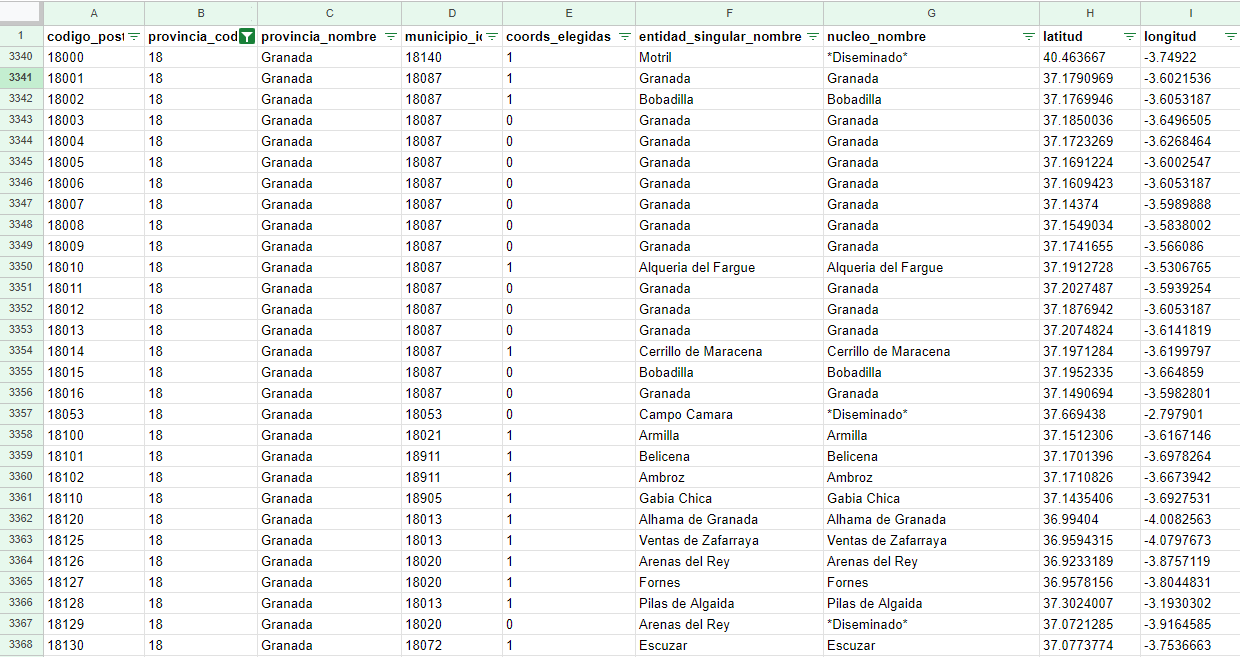
\includegraphics[height=70mm]{imagenes/municipios_cp.png}
    \caption{CSV con la información de códigos postales para la base de datos}
    \label{fig:CSV_municipios}
\end{figure}


\subsubsection{Visualización de los gastos en el mapa}
Para la representación de los gastos en el mapa se necesitan analizar las transacciones correspondientes a operaciones de gasto realizadas en el mes actual y extraer las coordenadas geográficas de los localidades para representarlos en un punto concreto en el mapa. 

Como solución se ha implementó un endpoint en el backend que obtiene los gastos por ubicación para el mes actual. Primero filtra las transacciones del mes y año actuales, agrupadas por código postal. Del resultado extrae cada código postal con el total de gastos asociado a él y le añade las coordenadas y nombres de localidades. Finalmente, devuelve una lista de gastos con coordenadas y nombres de entidades.

\begin{lstlisting} [language=Python, caption=Endpoint para obtener los gastos por localidad]
@app.get("/expenses_by_location", tags=["Map"], status_code=status.HTTP_200_OK)
def get_expenses_by_location(db: Session = Depends(get_db)):
    current_month = datetime.now().month
    current_year = datetime.now().year

    expenses_by_location_query = db.query(
        Transaction.shop_location_pc,
        func.coalesce(func.sum(Transaction.amount), 0).label('current_amount_spent')
    ).filter(
        Transaction.shop_location_pc != None,
        extract('month', Transaction.insert_date) == current_month,
        extract('year', Transaction.insert_date) == current_year
    ).group_by(Transaction.shop_location_pc).all()

    expenses_by_location = [row._asdict() for row in expenses_by_location_query]

    expenses_with_coordinates = []
    for expense in expenses_by_location:
        postal_code = expense['shop_location_pc']
        coordinates = get_location_by_postal_code(postal_code, db)
        if coordinates != {"desconocido"}:
            existing_expense = next((exp for exp in expenses_with_coordinates if exp['entidad_nombre'] == coordinates['entidad_nombre']), None)
            if existing_expense:
                existing_expense['current_amount_spent'] += expense['current_amount_spent']
                existing_expense['postal_codes'].append(postal_code)
            else:
                expense_by_loc = {
                    'postal_codes': [postal_code],
                    'latitude': coordinates['latitude'],
                    'longitude': coordinates['longitude'],
                    'entidad_nombre': coordinates['entidad_nombre'],
                    'current_amount_spent': expense['current_amount_spent']
                }
                expenses_with_coordinates.append(expense_by_loc)

    return expenses_with_coordinates
\end{lstlisting}

\begin{figure}[ht!]
    \centering
    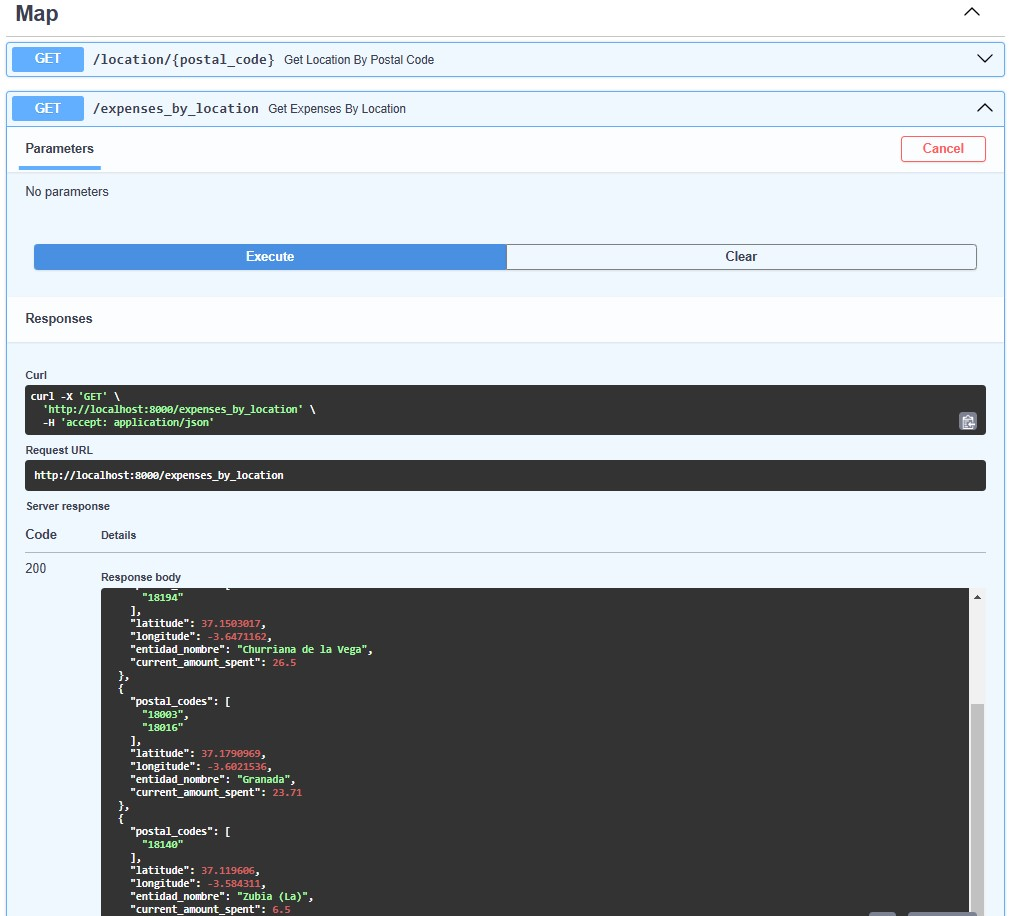
\includegraphics[width=\linewidth]{imagenes/api-expenses_by_location.jpg}
    \caption{Prueba del endpoint \textit{expenses\_by\_location} en la API de FastAPI a través de Swagger}
    \label{fig:api-expenses_by_location}
\end{figure}

\subsection{Mapa de gastos por comercio}
Para ofrecer un análisis geográfico más detallado de los gastos, se implementó la visualización sobre el mapa de gastos por tienda. Para ello, en los formularios de introducción de gastos se hizo visible un campo (no usado hasta el momento) para que el usuario pueda introducir la tienda donde realizó la compra. 

Este campo se completa seleccionando un item sobre una lista de tiendas predefinidas, evitando así la introducción manual de la dirección de la tienda y por tanto el sobreesfuerzo del usuario. Además, para facilitar la selección de la tienda, se implementó un componente en el frontend de un pequeño mapa para que el usuario verifique la ubicación de la tienda seleccionada.

Las información de tiendas se recoge en la base de datos en una tabla que se irá construyendo a medida que los usuarios vayan introduciendo comercios en la aplicación.


\subsubsection{Introducción de un comercio en la aplicación}
El usuario puede introducir una tienda en la aplicación de dos formas: por geolocalización o por búsqueda.

Ambos métodos parten del código postal introducido por el usuario en el formulario de gastos. El proceso para encontrar las tiendas difiere en la forma de obtener las coordenadas con las que iniciar la búsqueda. Cuando se consiguen dichas coordenadas, se contruye una consulta en el formato de de Overpass QL para buscar puntos de interés (nodos) que coincidan con el criterio de búsqueda que se haya configurado. La consulta se envía a la API de Overpass y se obtiene una respuesta en formato JSON con los resultados de la búsqueda. Devuelve información de establecimientos de la que se obtienen las coordenadas, calle, nombre e identificador del elemento para introducirlo, junto con el código postal, en la base de datos, creando una nueva entrada en la tabla de tiendas por medio de un endpoint de la API de Sigma.

\begin{itemize}
    \item Identificación de un comercio con buscador    
    En este caso, la consulta en el ???? ref ???? define diferentes filtros de búsqueda para encontrar elementos en OpenStreetMap con atributos que coincidan con el término de búsqueda (searchStr) y estén ubicados en el radio especificado (meters alrededor de lat, lon). Teniendo en cuenta que las coordenadas parten de un código postal, el radio debe ser lo suficientemente generoso para abarcar la zona completa (aunque suponga exceder el área real del código postal). Siendo:
    \subitem \textit{searchStr} el término de búsqueda introducido por el usuario
    \subitem \textit{meters} la distancia en metros alrededor de la ubicación del usuario
    \subitem \textit{lat, lon} las coordenadas geográficas asociadas al \textbf{código postal} completado en el formulario.
    
    \begin{lstlisting} [language=Python, caption=Consulta de Overpass QL con término de búsqueda]
    const overpassQuery = `
        [out:json];
        (
        node["name"~"${capitalize(searchStr)}"](around:${meters}, ${lat}, ${lon});
        node["shop"~"${capitalize(searchStr)}"](around:${meters}, ${lat}, ${lon});
        node["amenity"~"${capitalize(searchStr)}"](around:${meters}, ${lat}, ${lon});
        node["addr:street"~"${capitalize(searchStr)}"](around:${meters}, ${lat}, ${lon});
        );
        out body;
    `;
    \end{lstlisting}

    \item Introducción de un comercio con geolocalización 
    Concretamente, la obtención de las coordenadas alrededor de las cuales se buscarán los puntos de interés se realizó a partir de la geolocalización del usuario con la API de geolocalización de HTML5 a través de la biblioteca Leaflet Locatecontrol. Se construyó una consulta ????? ref ??? en Overpass QL que busca nodos (puntos de interés) en OpenStreetMap dentro de un área de proximidad mucho más reducida ya que utilizará las coordenadas exactas de la ubicación del usuario, se centra en un conjunto de etiquetas específicas y no utiliza un término de búsqueda concreto, ya que por la precisión de las coordenadas el número de comercios encontrados en el área, será reducido.
    \begin{lstlisting} [language=Python, caption=Consulta de Overpass QL con geolocalización]
    const overpassQuery = `
        [out:json];
        (
        node["name"](around:${meters}, ${lat}, ${lon});
        node["shop"](around:${meters}, ${lat}, ${lon});
        node["amenity"~"restaurant|cafe|bar|bank|pharmacy|post_office|fast_food|clinic|vending_machine"](around:400,${lat},${lon});
        node["addr:street"](around:${meters}, ${lat}, ${lon});               
        );
        out body;
    `;
    \end{lstlisting}

\end{itemize}

Finalmente, el usuario selecciona un comercio de la lista de resultados devuelta por la API de Overpass y ésta se añade a la base de datos de la aplicación. Para que el usuario pueda verificar la ubicación de la tienda seleccionada, se creó un componente para mostrar un pequeño mapa en el formulario de gastos donde aparece la tienda seleccionada.

\subsubsection{Visualización de los gastos en el mapa}
La representación de los gastos en el mapa se realiza de forma similar a la de los gastos por localidad. Tan solo cambia la consulta al backend, se creó un nuevo endpoint para obtener los gastos por tienda en lugar de por localidad. Se reutilizó el componente de React para mostrar, en este caso, el resultado de la consulta a la API que devuelve una lista donde cada elemento contiene las coordenadas geográficas, nombre de la tienda y cantidad total de gastos asociada.

\section{Pruebas}
Se realizaron diversas pruebas para comprobar el correcto funcionamiento de las funcionalidades implementadas y poder cerrar este milestone. 
Para verificar la implementación de la funcionalidad asociada a los mapas, realicé diversas pruebas usando DBeaver, Swagger de FastAPI y el frontend de la aplicación. Las pruebas fueron orientadas a garantizar el correcto flujo de datos y la visualización precisa de gastos en el mapa. A continuación, se resume el enfoque de las pruebas realizadas para esta funcionalidad:

\begin{itemize}
    \item Almacenamiento de Datos en la Base de Datos\\
     Verifiqué que los datos introducidos en los formularios del frontend (especialmente el código postal y la tienda) se almacenaban correctamente en la base de datos tras enviarse. Comprobé manualmente que cada registro reflejaba fielmente los datos ingresados.
    \item Pruebas de consulta a Endpoints con Swagger\\
     Probé cada endpoint de FastAPI relacionado con la funcionalidad de mapas (consultas de coordenadas dado un código postal, y de gastos por localidad o tienda). Verifiqué que las respuestas fueran precisas y completas, devolviendo datos en el formato JSON esperado.
    \item Visualización en Mapas (Frontend)\\
     En el frontend, revisé la vista de mapas para asegurar que los puntos de gasto se mostraran correctamente en el mapa de España. Verifiqué que la ubicación de los puntos coincidiera con la información de gastos agrupada por localidad o tienda, de acuerdo a los datos obtenidos desde la base de datos.
    \item Consultas a la API de Overpass\\
     Probé la integración con la API de Overpass para obtener información de tiendas cercanas a la ubicación del usuario (o código postal). Verifiqué que los datos retornados fueran precisos y se reflejaran adecuadamente en el mapa.
\end{itemize}

Esta combinación de pruebas manuales en la base de datos, el backend y el frontend permitió asegurar que la funcionalidad de mapas se implementara correctamente, facilitando al usuario la visualización intuitiva de sus gastos mensuales por localidades y tiendas.


\begin{figure}[ht!]
    \centering
    \begin{minipage}{0.45\textwidth}
        \centering
        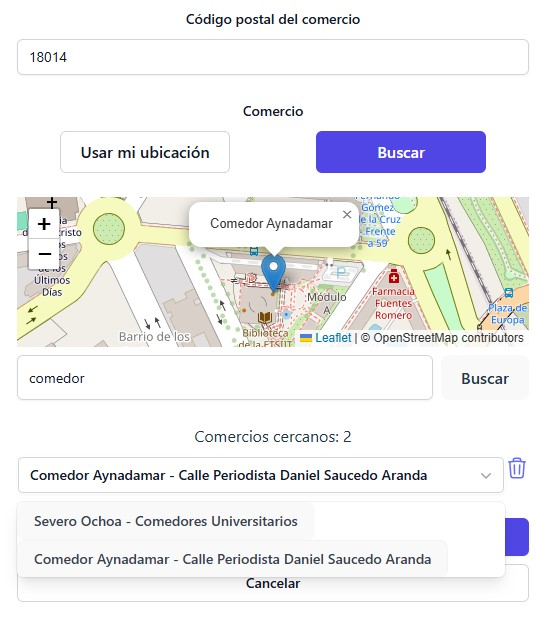
\includegraphics[height = 70mm]{imagenes/mapa_buscador_comercio.jpg}
        \caption{Búsqueda de comercio por buscador en el formulario de gastos}
        \label{fig:mapa_buscador_comercio}
    \end{minipage}\hfill
    \begin{minipage}{0.45\textwidth}
        \centering
        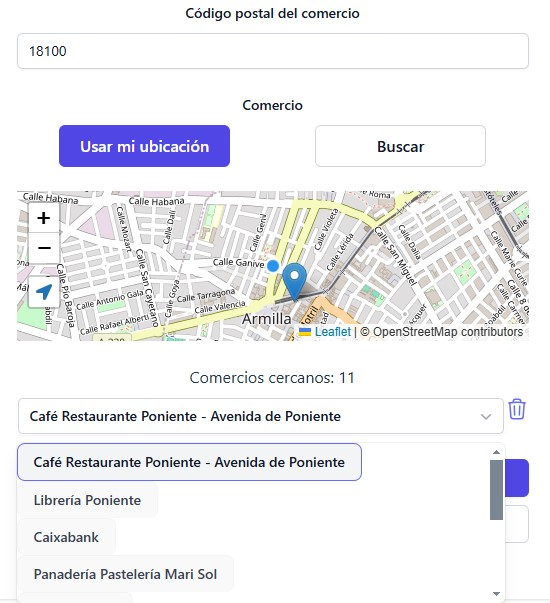
\includegraphics[height = 70mm]{imagenes/mapa_GPS_comercio.jpg}
        \caption{Búsqueda de comercio por geolocalización en el formulario de gastos}
        \label{fig:mapa_GPS_comercio}
    \end{minipage}
\end{figure}

\begin{figure}[ht!]
    \centering
    \begin{minipage}{0.45\textwidth}
        \centering
        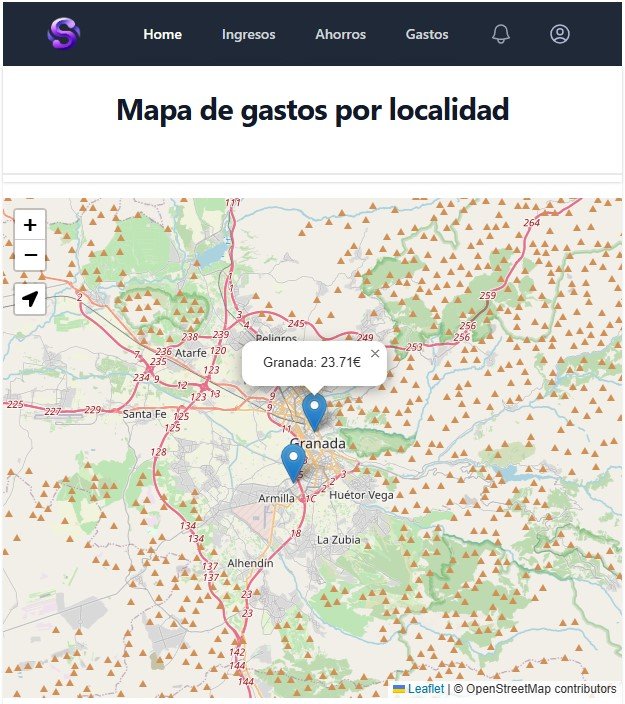
\includegraphics[height = 70mm]{imagenes/mapa_gasto_localidades.jpg}
        \caption{Mapa de gastos por localidad}
        \label{fig:mapa_gasto_localidades}
    \end{minipage}\hfill
    \begin{minipage}{0.45\textwidth}
        \centering
        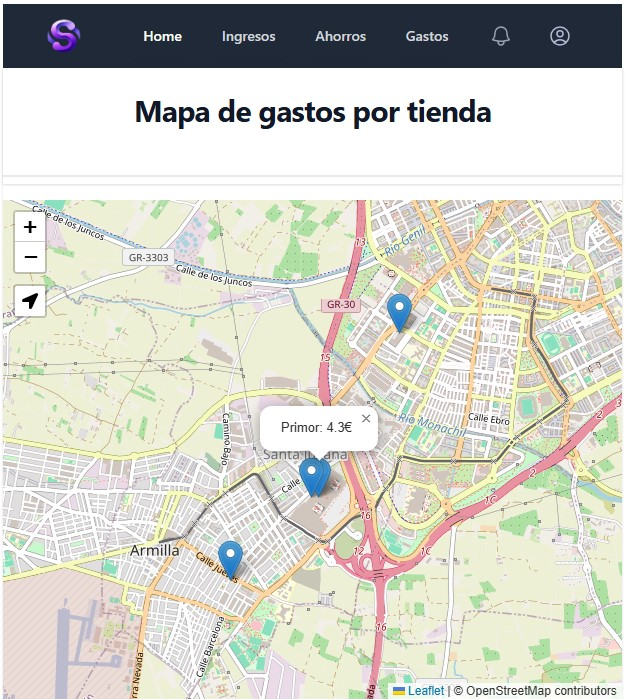
\includegraphics[height = 70mm]{imagenes/mapa_gasto_comercios.jpg}
        \caption{Mapa de gastos por comercio}
        \label{fig:mapa_gasto_comercios}
    \end{minipage}
\end{figure}

	% \input{secciones/08_costes}

	% Conclusiones
	\chapter{Conclusiones y trabajos futuros}

\section{Objetivos} \label{sect:goals}
\textit{El objetivo principal de este proyecto es desarrollar una aplicación web (\textbf{SIGMA}: Sistema Inteligente de Gestión Monetaria Automatizada) 
para la gestión financiera. Usando tecnologías de reconocimiento
óptico de caracteres (OCR) y geolocalización, permite al usuario llevar a cabo un 
análisis de gastos detallado y facilita una gestión eficiente de su dinero
a través de un monedero virtual, introduciendo los datos de 
forma sencilla.}

Para el cumplimiento de este objetivo general se plantean los siguientes objetivos específicos:
\begin{enumerate}
    \item Analizar las herramientas de gestión financiera existentes en el mercado para su aplicación en el desarrollo del proyecto.  
    \item Plantear un diseño escalable y desarrollar una arquitectura de software modular para facilitar la integración de futuras funcionalidades o mejoras. 
    \item Diseñar e implementar la interfaz de usuario para permitir la creación 
         de transacciones (ingresos, gastos y ahorros), categorías de gasto y objetivos de ahorro personalizables y modificables.
    \item Implementar herramientas de visualización de datos por medio de mapas, gráficos y resúmenes automatizados para analizar los patrones de gasto y realizar un seguimiento claro de los mismos.
    \item Estudiar e integrar tecnología de reconocimiento óptico de caracteres (OCR) y de reconocimiento de patrones en un texto para escanear tickets de compra; como punto de partida al procesamiento del texto obtenido.
    \item Implementar un sistema que permita automatizar la inserción de gastos en la aplicación, extrayendo datos relevantes de los tickets de compra para que la interverción por parte del usuario en el proceso sea mínima.
    \item Facilitar la búsqueda de comercios. Integrar en la aplicación capacidades de geolocalización para identificar en las transacciones el comercio en el que se ha realizado dicho gasto.   
    
\end{enumerate}

\section{Conclusiones}
\section{Conclusiones}
A lo largo del desarrollo de este proyecto, se han alcanzado satisfactoriamente los objetivos establecidos en la fase inicial. Estos objetivos sirvieron como guía para asegurar que cada funcionalidad cumpliera con los requerimientos del usuario y aportara una solución eficaz en el ámbito de la gestión financiera. A continuación, se detallan las conclusiones obtenidas en relación con cada uno de los objetivos planteados:

\begin{itemize}
    \item \textbf{Análisis de herramientas de gestión financiera}: El estudio de las herramientas existentes en el mercado permitió identificar las características y limitaciones más relevantes en el área de la gestión financiera personal. Gracias a este análisis, se establecieron funcionalidades clave para la aplicación, con un enfoque en simplicidad, usabilidad y flexibilidad.

    \item \textbf{Arquitectura modular y escalable}: Se ha diseñado e implementado una arquitectura de software modular, cumpliendo con el objetivo de facilitar la escalabilidad del proyecto. Esto asegura que futuras integraciones, como nuevas funcionalidades o mejoras en el rendimiento, puedan añadirse sin afectar a los componentes existentes. La arquitectura modular permite una mayor adaptabilidad a las necesidades de los usuarios a lo largo del tiempo.

    \item \textbf{Diseño de la interfaz de usuario}: La interfaz permite a los usuarios gestionar sus transacciones de ingresos, gastos y ahorros de manera eficiente. Se implementaron opciones para categorizar gastos y definir objetivos de ahorro personalizables, permitiendo a los usuarios tener un control claro sobre su situación financiera. Se cumple, por tanto, el objetivo de ofrecer una experiencia de usuario intuitiva y de bajo esfuerzo en la creación y modificación de transacciones y categorías.

    \item \textbf{Visualización de datos mediante gráficos, mapas y resúmenes}: El sistema de visualización de datos proporciona gráficos y resúmenes automáticos de gastos, ofreciendo a los usuarios un análisis visual y detallado de sus patrones de consumo. Además, la visualización de gastos en mapas ayuda a los usuarios a relacionar sus gastos con ubicaciones geográficas específicas, lo cual contribuye a una mejor comprensión y seguimiento de los hábitos de consumo.

    \item \textbf{Integración de tecnología OCR y procesamiento de tickets}: La integración de la tecnología OCR permite escanear tickets de compra y extraer toda la información del ticket de manera eficiente. Esta funcionalidad es el punto de partida hacia un procesamiento automatizado de los datos de los tickets, reduciendo la necesidad de intervención manual por parte del usuario. Este logro representa un avance en la automatización y precisión de la gestión de gastos.

    \item \textbf{Automatización en la inserción de gastos}: Se implementó un sistema de automatización que extrae los datos relevantes de los tickets de compra, lo que minimiza la intervención del usuario en el registro de sus gastos. Esto permite a los usuarios registrar sus gastos de forma rápida y cómoda, mejorando la eficiencia del proceso y cumpliendo así con el objetivo de facilitar la inserción de datos en la aplicación.

    \item \textbf{Geolocalización y búsqueda de comercios}: La integración de la funcionalidad de geolocalización permite identificar y registrar el comercio asociado a cada transacción en función de la ubicación. Esto facilita a los usuarios la identificación de sus transacciones por ubicación y les brinda información adicional a localizar sus gastos en los diferentes comercios. Esta funcionalidad contribuye a una mayor precisión y detalle en el análisis de gastos.

\end{itemize}

Por tanto, este proyecto ha logrado desarrollar una solución completa y eficiente en el ámbito de la gestión financiera personal, aportando una herramienta que integra tecnologías avanzadas y proporciona una experiencia de usuario optimizada. Esta aplicación representa una contribución al estado del arte en la gestión de finanzas personales, ya que combina funciones de análisis de datos, automatización y geolocalización, adaptadas a las necesidades de los usuarios.

Durante el desarrollo de este proyecto, he tenido la oportunidad de enriquecerme en múltiples aspectos. Crear esta solución desde cero y de manera autónoma me ha permitido mejorar significativamente mis habilidades de análisis, ya que fue necesario plantear una construcción completa en el inicio que tuviera sentido como una unidad, para poder evaluar y determinar con claridad las funcionalidades y restricciones necesarias en cada fase que se implementaría. Por otro lado, en la búsqueda de soluciones y en la implementación de las mismas, he tenido la oportunidad de aprender y aplicar nuevas tecnologías y herramientas, lo que ha ampliado mi conocimiento y experiencia en el desarrollo de aplicaciones web.

Además, fue particularmente gratificante encontrar una solución eficaz para una problemática que enfrentaba personalmente y descubrir que esta también resultaba útil para personas de mi entorno. Compartir y discutir los primeros planteamientos sobre la aplicación con otras personas me ayudó a refinar y enfocar las necesidades del proyecto, logrando una mejor comprensión de sus objetivos y una implementación más alineada con las expectativas de los usuarios.

Este proyecto representó un reto de principio a fin, que finalmente ha cumplido con las expectativas y me ha permitido adquirir una valiosa experiencia en el desarrollo de software, desde la concepción de la idea hasta la implementación de una solución funcional y eficiente. En resumen, esta experiencia me ha dejado no solo con nuevas competencias técnicas, sino también con una comprensión más amplia del proceso de desarrollo y de la utilidad de una solución bien diseñada desde el primer momento.


\section{Trabajos futuros}
...

En la actualidad, cada vez son más los comercios que ofrecen la posibilidad de recibir 
el ticket en formato digital. En un futuro probablemente todos los tickets serán 
digitales para reducir el impacto ambiental del uso del papel y abaratar costes.

Por lo que se incluirá en la aplicación la opción de escaneo de tickets digitales.


Versión gratuita no almacena tickets.
Versión de pago para amortizar el almacenaje, que sí permita almacenar todos los tickets.

	% Trabajos futuros


	
	\newpage
	\bibliography{bibliografia}
	\bibliographystyle{plain}
	
\end{document}
